%TODO Check if 470m or 473m distance between detector and target (or even decay tunnel)
\chapter{Experimental Setup} %\label{sec:ExperimentalSetup}
MicroBooNE marks the first experiment of the \gls{lartpc} based \gls{sbn} at \gls{fnal}. The detector is located in the \gls{bnb}. Since neutrinos lack electromagnetic charge, they can not be accelerated directly with any technology known to humanity. Thus a complex accelerator system is employed to produce high energy protons, which are then collided onto a target. The products of said collision then decay \ia into neutrinos. A site map of the \gls{bnb} beam line and MicroBooNE is shown in figure \ref{fig:MicroBooNELocation}. As the above description is rather rudimentary, I would like to give a more detailed insight into the \gls{bnb} in the following paragraphs. Thereafter, I will discuss the MicroBooNE detector and its various subsystems.
\begin{figure}[htbp]
    \centering
    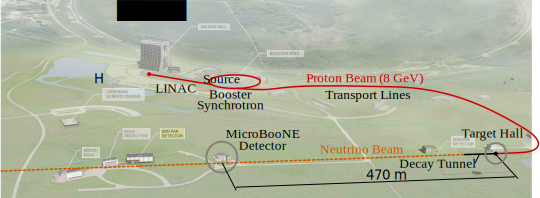
\includegraphics[width=1.0\textwidth]{images/MicroBooNE/MicroBooNELocation.pdf}
    \caption[Site map of the MicroBooNE Detector and the Booster Neutrino Beam Line]{Shown above is a site map of the MicroBooNE detector and the \gls{bnb} line. The beam line starts close to Wilson Hall at the \ce{H-} source (red dot). Then these ions and later protons are accelerated by the \gls{linac} and the Booster to \SI{8}{\giga\electronvolt} (red line). Thereafter transport lines (also red) guide the proton beam to the target (black dot). There the protons collide and produce, among other particles, pions and kaons. These then further decay into neutrinos and charged leptons in the decay tunnel (black line). The neutrinos traverse the rock (dashed orange line) and cross the detector after \SI{470}{\metre}. The original picture was sourced from \cite{MicroBooNEDetector} and modified.}
    \label{fig:MicroBooNELocation}
\end{figure}

\section{Booster Neutrino Beam} \label{sec:BNB}
Like many other high energy particle beams, the \gls{bnb}'s origin is an inconspicuous pressurised gas cylinder containing hydrogen gas, \ce{H2}. This hydrogen is then fed into a \textbf{dimpled magnetron} \cite{BNBProtonSource1,BNBProtonSource2}, where a dense plasma is produced. The electrons in the plasma are confined to spiral around the magnetron's cavity, while the protons are attracted by the cathode made of neodymium \cite{BNBProtonSource2}. A constantly reapplied caesium coating notably lowers the \gls{WorkFunction} of the cathode surface, such that the protons are able to acquire two electrons when impacting the surface. Thus, negatively charged hydrogen atoms, \ce{H-}, are formed which are then immediately repelled by the cathode \cite{BNBProtonSource1}. Through an aperture in the anode, the \ce{H-} ions are able to escape from the magnetron. In order to increase the efficiency of the \ce{H-} source, a spherical dimple is carved into the cathode opposite of the aperture, \ie said dimple has a focusing effect on the ions and facilitates their escape through the gap. In addition, a pulsed extractor cone, placed out side of the magnetron at the aperture, further increases the extraction yield and accelerates the \ce{H-} ions to a kinetic energy of \SI{35}{\kilo\electronvolt}. Said \ce{H-} extraction is pulsed to \SI{15}{\hertz} with a pulse width of \SI{230}{\micro\second} \cite{BNBProtonSource2,BNBProtonSource3}. From here, the low energy beam is guided into a four-rod \gls{rfq} injector, which is still considered part of the \ce{H-} source system. In principle the \gls{rfq} is a linear accelerator, within which an electromagnetic standing wave of \SI{201.25}{\mega\hertz} accelerates the \ce{H-} ions to a kinetic energy of \SI{750}{\kilo\electronvolt} \cite{BNBProtonSource4}. The beam current generated by above-described \ce{H-} source assembly is \SI{60}{\milli\ampere} \cite{BNBProtonSource3}. The \ce{H-} source is shown as a red dot, at the start of the proton beam line in figure \ref{fig:MicroBooNELocation}.

From the \ce{H-} source, the beam is transferred to the \gls{fnal} \gls{linac}, a series of linear particle accelerators. The \gls{linac} is comprised of five Alvarez drift tube cavities operated at \SI{201.24}{\mega\hertz} \cite{BNBLinac1} followed by seven high-frequency (\SI{805}{\mega\hertz}) side-coupled cavity structures \cite{BNBLinac2}. As the frequencies indicate, both technologies are powered by high-intensity radio waves, which induces an alternating electric field in these \gls{rf} cavities synchronised to the particle's motion. This way, the drift tube section accelerates the \ce{H-} beam to a kinetic energy of \SI{116.5}{\mega\electronvolt} while the side-coupled cavities increases their kinetic energy further to \SI{400}{\mega\electronvolt} \cite{BNBLinac3}. Naturally, the \gls{linac} is also pulsed to \SI{15}{\hertz} and synced to the \ce{H-} source cycles. These pulses are not to be confused with the beam bunches, \ie the fine structure of the pulses introduced by the cavity's \gls{rf}, \SI{805}{\mega\hertz} in the case of the \gls{linac}. The schematics of above-described \gls{linac} can be inferred from figure \ref{fig:Linac} and its location from figure \ref{fig:MicroBooNELocation}.
\begin{figure}[htbp]
    \centering
    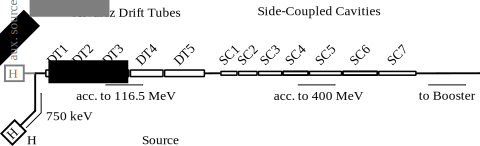
\includegraphics[width=1.0\textwidth]{images/MicroBooNE/LinacSchematics.pdf}
    \caption[Schematics View of the Linac]{This graph shows a schematics view of \gls{fnal} \gls{linac}. The \ce{H-} ions leave the source with an kinetic energy of \SI{750}{\kilo\electronvolt}. These ions are then first accelerated to \SI{116.5}{\mega\electronvolt} by Alvarez drift tubes (DT1 through DT5), and then further accelerated to \SI{400}{\mega\electronvolt} by side-coupled cavities (SC1 through SC7). This schematic view is inspired by \cite{BNBLinac3}.}
    \label{fig:Linac}
\end{figure}

Before the particles are accelerated further, they pass through a thin foil made of carbon. Said foil causes the stripping of all electrons from the \ce{H-} ions, thus yielding a pure proton beam \cite{BNBBooster1}. Thereafter, the protons are injected into the Booster synchrotron ring with a circumference of \SI{474.2}{\metre} \cite{BNBBooster2}. Acceleration in the Boster ring occurs in three steps \cite{BNBBooster1}:
\begin{enumerate}
    \item Injection from the \gls{linac}, and bunching within \SI{2}{\milli\second}.
    \item Acceleration, lasting about \SI{29}{\milli\second}.
    \item Eventual phase locking with the next accelerator stage and extraction in \SI{2.5}{\milli\second}.
\end{enumerate}
Above cycle is repeated every \SI{1/15}{\second}, in sync with the \gls{linac} injection of \SI{15}{\hertz}. In the injection phase, the proton's energy spread of about \SI{0.3}{\percent}, introduced by the \gls{linac}, is first reduced and with it, the \gls{linac}'s \SI{805}{\mega\hertz} bunch structure disappears as well. The Booster ring features \num{17} ferrite-tuned resonator \gls{rf} cavities as accelerators located in one half of the ring. In contrast to the \gls{linac} and the \gls{rfq}, these Booster cavities feature variable frequencies. Right after injection, the Booster's \gls{rf} cavities operate at \SI{37.86}{\mega\hertz} and the \SI{400}{\mega\electronvolt} proton beam requires \SI{2.2}{\micro\second} to complete a full revolution of the ring. Dipole magnets along the sychrotron's circumference keep the beam in its orbit. In order to increase the kinetic energy of the protons, the frequency in the \gls{rf} cavities needs to be raised slowly and with it, the magnetic field of the dipoles in order to stabilise the beam on its trajectory. At the end of the \SI{29}{\milli\second} acceleration cycle, the cavity frequency reaches \SI{52.81}{\mega\hertz}. In this process the proton kinetic energy reaches \SI{8}{\giga\electronvolt} and the full ring revolution time is reduced to \SI{1.6}{\micro\second}. The latter also gives us the pulse width of the beam, while it contains \num{84} bunches given by the frequency of the cavities. Since the \gls{bnb} does not use higher energy protons than the ones provided by the Booster, the phase locking before extraction is not required. The extraction of the beam from the synchrotron ring is accomplished by fast switching magnets (\SI{40}{\nano\second} rise time), called \textbf{kickers}. During the whole acceleration process, a multitude of beam optics magnets is used to stabilise the beam on its trajectory. All the aforementioned Booster properties are sourced from \cite{BNBBooster1,BNBBooster2}. The location of the Booster synchrotron can be extracted from figure \ref{fig:MicroBooNELocation}.

From the Booster, the \SI{8}{\giga\electronvolt} proton beam pulses are guided with a frequency of \SI{15}{\hertz} to the various experiments or to additional accelerators. In the \gls{bnb}'s case, at most every third Booster pulse is routed through transport lines and various beam optics elements to the target hall, as indicated in figure \ref{fig:MicroBooNELocation}. This leads to a \gls{bnb} beam pulse frequency of $f_\text{BNB} \leq \SI{5}{\hertz}$. At the target hall, the proton beam is extracted from beam vacuum pipes into air and after \SI{1.5}{\metre} collided onto a beryllium target \cite{BNBBeamFlux}. The full target assembly is shown in figure \ref{fig:BNBTarget}.
\begin{figure}[htbp]
    \centering
    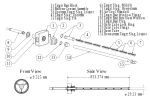
\includegraphics[width=1.0\textwidth]{images/MicroBooNE/BNBTarget.pdf}
    \caption[Technical Drawing of the BNB Target]{This figure depicts a technical drawing of the \gls{bnb} beryllium target, sourced from \cite{BNBBeamFlux}. In the side view, the proton beam hits the target from the left hand side.}
    \label{fig:BNBTarget}
\end{figure}
This main target structure is composed of seven identical so-called \textbf{target slugs} placed in a row along the proton beam axis. These slugs are beryllium cylinders with a diameter of \SI{9.525}{\milli\metre} featuring three regularly spaced fins. Said fins hold the target in the centre of a surrounding tube and provide air-cooling. Beryllium is chosen because of its relatively low atomic number, $Z$, and its low density, $\rho$, which lead to a low \textbf{linear stopping power} for charged particles according to the \textbf{Bethe equation} \ref{eq:BetheBloch}. This is advantageous as the aim is to spend most of the energy as possible for neutrino production rather than ionisation. Furthermore, beryllium features low residual radioactivity after being exposed to a proton beam and it allows for air cooling, reducing the complexity of the target system \cite{BNBBeamFlux}. Before the collision, the proton beam gets focused on the cylindrical part of the upstream target slug. This leads to maximum collision yield of \num{5e12} \gls{pot} per beam pulse \cite{BNBBeamFlux}. 

The above-described target assembly is embedded into a so-called \textbf{horn electromagnet}. Said horn is, simply put, a hollow cylinder with electrically conducting surfaces. At the upstream end of the cylinder, the inner and outer surfaces are electrically insulated. Now, if power is applied across said insulation, a current will flow from the inner conductor layer to the outer in neutrino mode or vice-versa in anti-neutrino. This current then induces a toroidal magnetic field, $\vec{B}$, which falls with $1/R$, where $R$ is the radial distance from the cylinder axis. A cutaway view of the above described horn electromagnet is shown in figure \ref{fig:BNBNeutrinoProduction}. The \gls{bnb} horn is composed of an aluminium alloy. The horn's current is pulsed to \SI{5}{\hertz} with a pulse length amounting to \SI{143}{\micro\second}. Naturally, the current pulse is synchronised with the arrival of the Booster proton beam. At its peak the horn current reaches \SI{174(1)}{\kilo\ampere}, resulting in a maximum magnetic field strength $B_\text{max} = \SI{1.5}{\tesla}$ \cite{BNBBeamFlux}. The \gls{bnb} horn is situated in front of a \SI{45}{\metre} long air-filled decay tunnel, also shown in figure \ref{fig:BNBNeutrinoProduction}. From the upstream face of the target to the beam stop at the end of the decay tunnel the distance amounts to \SI{50}{\metre}.
\begin{figure}[htbp]
    \centering
    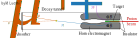
\includegraphics[width=1.0\textwidth]{images/MicroBooNE/BNBNeutrinoProduction.pdf}
    \caption[Neutrino Production Process at the BNB Target Hall]{This figure shows a schematic view of the neutrino production facility located at the target hall (not to scale), sourced from \cite{LArLaserPhDMatthias}. The drawing is cylindrically symmetrical along the proton beam axis. Here, the beryllium target (green) is inserted into a horn electromagnet (grey). The annular electrical insulation of the horn assembly is shown as brown spots. The aforementioned target and horn assembly is then placed in front of a \SI{45}{\metre} long decay tunnel. Now, if the proton beam (red) hits the target, a host of secondary particles are produced, here indicated by pions, $\pi^+$ (blue) and $\pi^-$ (purple). In the picture, the horn's magnetic field, $\vec{B}$, is polarised in neutrino mode. Hence positively charged particles are focused forward into the decay tunnel, while negatively charged particles are deflected to the side. In the decay tunnel, $\pi^+$ decays into a muon, $\mu$ (solid orange), and its neutrino, $\nu_\mu$ (dashed orange). Finally, most of the muons are stopped in the absorber where they decay.}
    \label{fig:BNBNeutrinoProduction}
\end{figure}

The primary \SI{8}{\giga\electronvolt} Booster protons produce a multitude of secondary particles interacting with the beryllium. These secondaries are predominantly composed of pions, $\pi^{\pm}$, charged kaons, $K^{\pm}$, neutral kaons, $K^0$, protons, $p$, and neutrons, $n$. Their respective production rate per proton-beryllium interaction is listed in table \ref{tab:BNBSecondaryComposition}.
\begin{table}[htbp]
    \centering
    \caption[BNB Secondary Particle Composition after Target Interaction]{This table lists the secondary particle composition after a single \SI{8}{\giga\electronvolt} proton-beryllium interaction in the \gls{bnb} target. Furthermore, the average secondary particle momentum, $\langle p \rangle$, and their average angle with respect to the primary proton beam axis, $\langle \theta \rangle$, are presented. This data is based on a \gls{mc} simulation performed for the MiniBooNE experiment \cite{BNBBeamFlux} and thus has to viewed with some healthy scepticism.}
    \begin{tabu} to 0.7\textwidth{X[-0.5c] X[c] X[-0.5c] X[-0.5c]} \toprule
        Secondary Particle & Multiplicity per \ce{$p$-Be} reaction & $\langle p \rangle$ $[\si{\giga\electronvolt\per\lightspeed}]$ & $\langle \theta \rangle$ $[\si{\milli\radian}]$ \\ \midrule
        $p$ & 1.5462 & 2.64 & 441 \\
        $n$ & 1.3434 & 1.59 & 586 \\
        $\pi^-$ & 0.9004 & 0.82 & 556 \\
        $\pi^+$ & 0.8825 & 1.11 & 412 \\
        $K^+$ & 0.0689 & 1.69 & 332 \\
        $K^0$ & 0.0241 & 1.34 & 414 \\
        $K^-$ & 0.0024 & 1.26 & 259\\ \bottomrule
    \end{tabu}
    \label{tab:BNBSecondaryComposition}
\end{table}
Of these secondary particles, only the \glspl{Meson} are of interest, since the baryonic secondaries, \ie $p$ and $n$, are not able to contribute to the neutrino production, due to their long lifetime. As the aforementioned table indicates, the substantial majority ($\sim \SI{95}{\percent}$) of secondary \glspl{Meson} are given by the charged pions. After their creation, most of the secondary pions scatter out of the beryllium target slugs with an average angle from the primary proton beam of $\langle \theta \rangle \approx \SI{24}{\degree}$ for $\pi^+$, and $\langle \theta \rangle \approx \SI{32}{\degree}$ for $\pi^-$, respectively. As they enter the horn electromagnet, they become subject to the strong magnetic field. Depending on the polarisation of the horn, one of the charges gets focused forward into the decay tunnel, while the opposite charge is deflected to the sides, as shown in figure \ref{fig:BNBNeutrinoProduction}. In neutrino mode, the horn's polarisation is such that $\pi^+$ are focused, while the $\pi^-$ are deflected. Since my thesis contains solely neutrino cross section measurements, I will omit the anti-neutrino mode from here on out.

Once in the decay tunnel, most of the positively charged secondary \glspl{Meson} decay in flight \ia into neutrinos. As an example for this process let us consider the decay modes of the two most prominent contributors \cite{PDG2018}
\begin{align}
    \ce{$\pi^{+}$ &->[\SI{99.99}{\percent}] $\mu^{+}$ +  $\nu_{\mu}$} \\
    \ce{$K^{+}$ &->[\SI{63.56}{\percent}] $\mu^{+}$ +  $\nu_{\mu}$}. \nonumber
\end{align}
Here the percentage denotes the fraction of said decay channel. The relatively high momentum of the secondaries, \ie average momentum $\langle p \rangle > \SI{1}{\giga\electronvolt}$, means that most of these secondary \glspl{Meson} are relativistic particles with a notable \textbf{Lorentz boost}. Thus, the decay products are focused forward when viewed in a reference frame at rest, as is the case here. In fact, it is these \textbf{Lorentz boosted} decay neutrinos which constitute the \gls{bnb}. Said neutrinos then traverses the rock due to the small interaction cross section. All the charged massive remnants of the above-described neutrino beam production process eventually loose their energy in the absorber and decay there at rest. The in flight decay process of a $\pi^+$ is also illustrated in figure \ref{fig:BNBNeutrinoProduction}.

So far we considered only the ideal neutrino production process, but in reality it is impossible to create a single flavour neutrino beam. Smart design choices, however, are able to reduce beam contaminants, \ie neutrinos of different flavour. The \SI{50}{\metre} decay distance, for instance, is optimised for allowing most $\pi^\pm$ and $K^\pm$ to decay within their typical lifetime of $\mathcal{O}(\SI{e-8}{\second})$), while preventing muon decays with a lifetime of $\mathcal{O}(\SI{e-6}{\second})$. The latter contaminate the beam with their two-neutrino decay signature \cite{PDG2018},
\begin{equation}
    \ce{$\mu^{+}$ ->[$\sim\SI{100}{\percent}$] $e^{+}$ + $\nu_{e}$ + $\bar{\nu}_{\mu}$}.
\end{equation}
The fact that most muons are stopped in the absorber, leads to a reduction of contaminants in the \gls{bnb}, as possible neutrinos originating from above decay at rest are not Lorentz boosted and thus radiate homogenously in all directions. Yet, the $\mu^+$ decays contribute the majority of $\nu_e$ contaminants in the \gls{bnb} \cite{BNBBeamFlux}. Another crucial design element, in regard of contaminants, is the horn electromagnet, which is responsible for deflecting the negatively charged secondaries. Then the horn is not able to deflect particles which stay within its inner conductor layer. Accordingly, the $\bar{\nu}_\mu$ beam impurity is introduced predominantly by the $\pi^-$ decay \cite{PDG2018},
\begin{equation}
    \ce{$\pi^{-}$ ->[\SI{99.99}{\percent}] $\mu^{-}$ +  $\bar{\nu}_{\mu}$}.
\end{equation}
According to simulations $\bar{\nu}_\mu$ represents the largest proportion of contaminants in the \gls{bnb} in neutrino mode with almost \SI{6}{\percent}, see table \ref{tab:BNBFluxComposition}. 
\begin{table}[htbp]
    \centering
    \caption[BNB Integrated Flux Composition]{Listed here is the expected \gls{bnb} integrated flux composition by neutrino flavour in neutrino mode at the MicroBooNE location. In neutrino mode, all neutrino flavours other than $\nu_\mu$ are considered beam contaminants or impurities. The beam fluxes presented here are the integrals of the graphs in figure \ref{fig:BNBFlux} and are sourced from \cite{BNBBeamUncertainty}.}
    \begin{tabu} to 0.6\textwidth{X[-0.4c] X[1.0c] X[-0.5c]} \toprule
        Neutrino Flavour & Integrated Flux $[\si{\per\centi\metre\squared\per\pot}]$ & Fraction $[\si{\percent}]$ \\ \midrule
        $\nu_\mu$ & \num{7.18(90)e-10} & \num{93.63} \\
        $\bar{\nu}_\mu$ & \num{4.45(60)e-11} & \num{5.81} \\
        $\nu_e$ & \num{3.91(46)e-12} & \num{0.51} \\
        $\bar{\nu}_e$ & \num{3.93(77)e-13} & \num{0.05} \\ \bottomrule
    \end{tabu}
    \label{tab:BNBFluxComposition}
\end{table}
Another impurity source are neutral particles, in particular $K^0_L$. As neutral particles do not exhibit any electrical charge, they obviously are not subject to the \textbf{Lorentz force} and thus are not affected by the horn. Hence, $K^0_L$ particles mostly stay on their trajectory after leaving the target with an average energy of \SI{1.24}{\giga\electronvolt} and an average angle of $\sim\SI{24}{\degree}$. Notably, the $K^0_L$ decay channel \cite{PDG2018},
\begin{equation}
    \ce{$K^{0}_{L}$ ->[\SI{20.28}{\percent}] $\pi^{+}$ + $e^-$ + $\bar{\nu}_{e}$},
\end{equation}
is the major contributor to $\bar{\nu}_{e}$ impurities in the \gls{bnb}, again according to simulations \cite{BNBBeamFlux}. The total neutrino fluxes of the four relevant flavours at MicroBooNE's location are listed in table \ref{tab:BNBFluxComposition} and their energy dependence, including uncertainties, are shown in figure \ref{fig:BNBFlux}.
\begin{figure}[htbp]
    \centering
    \includegraphics[width=1.0\textwidth]{images/MicroBooNE/BNBFluxMicroBooNE.pdf}
    \caption[BNB Flux in Neutrino Mode at MicroBooNE]{Shown here is the \gls{bnb} flux $\Phi(E_\nu)$ in neutrino mode for various neutrino flavours, $\nu_\mu$, $\bar{\nu}_\mu$, $\nu_e$, and $\bar{\nu}_e$, at the location of the MicroBooNE detector. These graphs are not measurements, but mere \gls{mc} simulation results and are thus subject to systematic uncertainties between \SIlist{6;26}{\percent} for $\nu_\mu$ and depending on the energy \cite{BNBBeamFlux,BNBBeamUncertainty}. The overall uncertainties are indicated by the coloured areas around the histograms.}
    \label{fig:BNBFlux}
\end{figure}

After the secondary \gls{Meson} decay and the charged particle absorption at the end of the decay tunnel, the neutrino beam (\gls{bnb}) traverses the ground material on its trajectory, as indicated by the orange dashed line in figure \ref{fig:MicroBooNELocation}. At a distance of \SI{470}{\metre} from the target, the \gls{bnb} crosses the MicroBooNE detector \cite{MicroBooNEDetector}. As discussed in section \ref{sec:CrossSectionCalculation}, the neutrino interaction cross section is extremely small, wherefore only a tiny fraction of the neutrinos generated in above-described process are able to interact, either in the detector or in the surrounding dirt. Side note: The dirt interaction also contribute to the background and are called dirt neutrinos. In neutrino mode the $\nu_\mu$-flux features a peak around \SI{600}{\mega\electronvolt} with a maximum of $\sim \SI{6e-10}{\per\centi\metre\squared\per\giga\electronvolt\per\pot}$ at MicroBooNE's location. The mean energy of the neutrinos is expected to be around \SI{820}{\mega\electronvolt}. The contaminant neutrino fluxes, have their maximum at energies below \SI{100}{\mega\electronvolt} and drop off with higher energies, see figure \ref{fig:BNBFlux}. Note, that \gls{bnb}'s pulse width, as its parent proton beam before, amounts to \SI{1.6}{\micro\second}.

% TODO check this again, appearently this has been done, but not at the right energies. The simulation is based on extrapolated data from beryllium interactions measured with the exact same target as the BNB is using!!! Yifan knows more about that!
Admittedly, in the neutrino flux lies one of the major deficiencies of all \gls{sbn} experiments, for the flux prediction is solely based on \gls{mc} simulations. This leads to large systematic uncertainties, \ie from \SIrange{6}{26}{\percent} for the energy dependent $\nu_\mu$-flux and \SI{12.5}{\percent} for the integrated $\nu_\mu$-flux \cite{BNBBeamUncertainty}. Chief contributor to these uncertainties are the hadronic interaction models of the Booster proton beam interacting with the beryllium target. They are based on a limited set of measurements, which had to be extrapolated in certain energy regions \cite{BNBBeamFlux}. These uncertainties could be minimised by dedicated measurements of the hadron flux emitted by the target assembly used for the \gls{bnb}. In my view, a measurement setup similar to the NA61/Shi$\nu$e experiment \cite{NA61Shine} is necessary to tackle said problem, but sadly there seems little interest in such a venture.

\section{MicroBooNE Cryogenic System}
MicroBooNE's cryogenic system consist of four main subsystems: the cryostat, which houses the \gls{lartpc} detector, the \gls{lar} purification system, the nitrogen refrigeration system, and a control and monitoring system. All cryogenic subsystems are interconnected by \SI{2.54}{\centi\metre} piping, insulated by \SI{10.2}{\centi\metre} of polyurethane foam. Where possible, \gls{cf} flanges with copper seals are used as piping connectors. In some cases, spiral-wound graphite gaskets are installed and smaller connection are made with VCR fittings using stainless steel gaskets. MicroBooNE's cryogenic system is based on the \gls{lapd} experiment \cite{LAPDPaper} and thereof derived experiences. Using \gls{lar} as a detector material requires a sophisticated cryogenic infrastructure, which is able to maintain stable conditions during long term measurements. Most importantly the argon has to be kept liquid, and therefore the heat input needs to be lower than the cooling power of the refrigeration system. Also, bubble formation and convection zones should be minimised, which is also synonymous with a low heat input and a small temperature gradient. The latter is important for providing a uniform drift velocity as well as a constant refractive index for \gls{uv} laser operations. Moreover, the system needs to be hermetically sealed (vacuum tight) in order to avoid rising impurity levels. Electronegative bonds which affect charge lifetime, like \ce{H2O} and \ce{O2}, can be reduced by copper filters, but \ce{N2} impurities, affecting the scintillation light yield, partly boil off at \gls{lar} temperatures and form an equilibrium. A schematic view of MicroBooNE's cryogenic system is depicted as a flow diagram in figure \ref{fig:CryoSystem}.
\begin{figure}[htbp]
    \centering
    \includegraphics[width=1.0\textwidth]{images/MicroBooNE/CryoSystem.pdf}
    \caption[Flow Diagram of MicroBooNE's Cryogenic System]{This figure shows the flow diagram of MicroBooNE's cryogenic system. Dashed lines represent gas lines while solid lines represent liquid lines. The colour blue stands for argon, green for nitrogen, and yellow for a 39:1 hydrogen-argon gas mixture used for filter regeneration. Picture sourced from \cite{MicroBooNEDetector}.}
    \label{fig:CryoSystem}
\end{figure}

The cryostat contains the whole detector setup of MicroBooNE. It is a grade \num{304} stainless steel vessel in a cylindrical shape with an inner diameter of \SI{381}{\centi\metre}, a length of \SI{1220}{\centi\metre} and a \SI{1.11}{\centi\metre} wall thickness, see figure \ref{fig:BareCryostat}. At each end the cryostat is covered by a domed cap. One of these caps was removed for the \gls{lartpc} and light readout system installation and thereafter welded back on. Protruding out of the cryostat vessle are \num{34} mostly \gls{cf} flanged nozzles. These allow for the insertion of various instruments, the placement of signal and \gls{hv} feedthroughs, as well as the exchange of liquid and gas argon with other cryogenic subsystem. The cryostat is placed on two supports made of wood in order to reduce the heat input through this important structure. In addition the whole cryostat surface was thermally insulated with a \SI{41}{\centi\metre} layer of spray-on closed cell polyurethane, as depicted in figure \ref{fig:InsulatedCryostat}. In the fully assembled and insulated configuration the cryostat is capable of containing \SI{170}{\tonne} of \gls{lar} at a maximum overpressure of \SI{2.1}{\bar} and a maximum heat load below \SI{15}{\watt\per\square\metre} \cite{MicroBooNEDetector}.
\begin{figure}[htbp]
    \centering
    \includegraphics[width=1.0\textwidth]{images/MicroBooNE/CryostatMicheleForScale.jpg}
    \caption[Bare MicroBooNE Cryostat]{This photograph shows the bare MicroBooNE cryostat with a professor for scale. The protruding nozzles are also visible, although many of them are wrapped in protective plastic. In the right bottom corner of the image, a part of the removed end cap of the cryostat is also visible.}
    \label{fig:BareCryostat}
\end{figure}
\begin{figure}[htbp]
    \centering
    \includegraphics[width=1.0\textwidth]{images/MicroBooNE/CryostatInsulated.jpg}
    \caption[Thermally Insulated MicroBooNE Cryostat]{Shown here is the cryostat after the spray-on thermal insulation of closed cell polyurethane was applied. The vessel rests on two wooden supports at its final position in the \gls{bnb}. This picture is sourced from \cite{MicroBooNEDetector}.}
    \label{fig:InsulatedCryostat}
\end{figure}

The purification system, is used to recirculate the \gls{lar} through filters in order to remove impurities with high \gls{electronegativity}. The filtered \gls{lar} then flows back to the cryostat. MicroBooNE's purification systems consists of two redundant filter lines in order to allow for one to be serviced during detector operations. For \gls{lar} recirculation, two Barber-Nichols BNCP-32B-000 magnetically-driven partial-emission centrifugal pumps are employed. The motor of this pump is mechanically decoupled from the impeller and the torque is transmitted by magnetic coupling. Thereby, the impeller's bearing is lubricated by the \gls{lar} itself, which prevents the contamination of \gls{lar} by washed-out lubricants. A single filter line consist of two different main filter stages enclosed by identical vacuum insulated \SI{77}{\litre} filtration beds. The first container in the \gls{lar} stream is filled with a molecular sieve featuring a pore diameter of \SI{4}{\angstrom} supplied by Sigma-Aldrich. This material primarily removes \ce{H2O} impurities, but also small amounts of \ce{N2} and \ce{O2}. The second filter stage contains pellets of BASF CU-0226S, consisting of highly dispersed copper oxide, \ce{CuO}, impregnated on a large-surface-area alumina. This stage removes mainly \ce{O2} and to a lesser extent \ce{H2O} as well. In order to be effective as a filter material, the \ce{CuO} needs to be activated by reducing it to \ce{Cu}. This can be achieved by a flow of a 39:1 \ce{Ar} and \ce{H2} gas mixture heated to \SI{473}{\kelvin}. While the reduction process only involves hydrogen \cite{LArFilterRegeneration}, \ie
\begin{equation}
    \ce{CuO + H2 ->[\SI{473}{\kelvin}] Cu + H2O},
\end{equation}
the inert argon gas serves as a fire suppressant. Pure heated \ce{H2} would be a fire hazard when exhausted into air. After this, the resulting water vapour of the reaction process is flushed out of the filter assembly by the applied gas pressure. The same procedure is also performed to regenerate the filters in regular intervals. At the outlet of the filter beds a \SI{10}{\micro\metre} sieve, made of sintered stainless steel prevents any small debris from flowing back to the cryostat. The primary requirements of the \gls{lar} purification system is to maintain the level of \ce{O2}-equivalent impurity levels below \SI{0.1}{\ppm}, in order to keep the loss of drift electrons below \SI{20}{\percent} over the full drift distance of the \gls{lartpc}. Moreover, the \ce{N2} contamination in \gls{lar} must be maintained below \SI{2}{\ppm}. This guaranties a negligible attenuation of scintillation photons within the active volume. In order to achieve these design goals, the \gls{lar} volume is fully recirculated and purified within \num{2.5} days.

Although the cryostat, the purification system, and piping are thermally insulated, the whole cryogenic system is subject to about \SI{\sim 3.9}{\kilo\watt} of heat load with the purification system offline, or \SI{\sim 6.0}{\kilo\watt} with operational purification system, respectively. Therefore two redundant liquid nitrogen refrigeration systems, with a cooling power of \SI{9.5}{\kilo\watt} each, are in place to take this heat out of the system. One unit consist of a cryogenic condenser, which is cooled by boiling off liquid nitrogen in a separated loop. During normal operations (with all systems online) a total of \SI{3400}{\liter} of liquid nitrogen are evaporated per day. During the refrigeration cycle, the heated gas argon is taken directly from the cryostat's gas phase and the resulting \gls{lar} is reintroduced to the systems in front of the recirculation pumps, see figure \ref{fig:CryoSystem}. This gets rid of impurities introduced during condensation.

Finally, the control and monitoring system consist of various sensors measuring \ia temperature and pressure located throughout the cryogenic system. The central piece, however, is the purity monitor system, consisting of three purity monitors of various drift lengths. Their design is based on the work of G. Carugno \etal \cite{LArPurityMonitor}. Said purity monitors are able to directly measure $Q/Q_0$, as discussed in section \ref{sec:ChargeDrift}, and provide accurate oxygen equivalent impurity level information in the range from \SIrange{0.3}{0.05}{\ppb} \cite{MicroBooNEDetector}. Accurate contamination measurements are paramount for stable \gls{lartpc} operations as it is an indicator for when to regenerate the filter system. A list of all primary design requirements for MicroBooNE's cryogenic system can be found in table \ref{tab:cryoreq}.
\begin{table}[htbp]
   \centering
   \caption[Primary Design Requirements for the Cryogenic and Purification Systems]{Primary design requirements for MicroBooNE's cryogenic and purification systems \cite{MicroBooNEDetector}.} 
    \begin{tabu}{lll}
    \toprule
    \rowfont[c]{\bf} Parameter & Value & Motivation\\
    \midrule
      \ce{O2}-equiv. impurity level & \SI{< 0.1}{\ppb} & MIP identification at full drift\\
      \ce{N2} impurity level & \SI{< 2}{\ppm} & Scintillation light output\\
      \gls{lar} temperature gradient & \SI{< 0.1}{\kelvin} & Drift-velocity uniformity\\
      \gls{lar} recirculation rate & 1 cryo-vol. $/$ \num{2.5} days & Maintain purity\\
      Cryostat heat load & \SI{< 15}{\watt\per\square\metre} & Min. convection and bubbles\\
      Cryogenic cooling capacity & \SI{10}{\kilo\watt} & Control expected heat load\\
      Max. operating pressure & \SI{2.1}{\bar} & Determines relief sizing\\
      \bottomrule
   \end{tabu}
   \label{tab:cryoreq}
\end{table}
% TODO Criticism of the cryo-system (maybe in a separate chapter)?

\section{MicroBooNE Detector} \label{sec:MicroBooNEDetector}
MicroBooNE employs a cuboid shaped \gls{lartpc}, see chapter \ref{sec:LArTPC}, with dimensions of \SI{2.560}{\metre} horizontal (drift) $\times$ \SI{2.325}{\metre} (vertical) $\times$ \SI{10.368}{\metre} (beam direction). The volume enclosed by the \gls{lartpc} is referred to as drift volume or active volume and amounts to \SI{61.71}{\metre\cubed}. Moreover, the mass of the \gls{lar} enclosed in the active volume is called \textbf{active mass}, which is expected to be \SI{86.15}{\tonne} if the argon is kept at its \gls{bp} at a pressure of \SI{1}{\bar}. On two sides, the active volume is confined by the anode and the cathode, which are parallel to each other and separated by \SI{2.56}{\metre}. The anode is formed by three readout wire planes and the cathode by nine stainless steel sheets with \SI{3.2}{\milli\metre} thickness. On the top, bottom, upstream, and downstream end, \num{64} field cage loops enclose the active volume in shape of rectangles with rounded corners. Each field cage loop consists of stainless steel tubes with a width of \SI{2.56}{\centi\metre}. The center-to-center distance between adjacent loops amounts to \SI{4.0}{\centi\metre}, leaving a gap of \SI{1.44}{\centi\metre} between them. Multiple electrically insulating \gls{G10} bars spanning the distance between anode and cathode hold the field cage loops in place. The structural integrity of the anode and cathode, respectively, arise from structural frames, also made of stainless steel. The detector is located at the \gls{lartf} at \gls{fnal}, about \SI{6}{\metre} below grade, in a pit without notable overburden. MicroBooNE's \gls{tpc} is shown in figure \ref{fig:MicroBooNETPC}.
\begin{figure}[htbp]
    \centering
    \subfloat[TPC View from the Cathode Side][\Gls{tpc} from the cathode side]
    {
        \includegraphics[width=0.48\textwidth]{images/MicroBooNE/TPCCathodeSide.jpg}
        \label{fig:MicroBooNETPCCathode}
    }
    \subfloat[TPC View from the Anode Side][\Gls{tpc} from the anode side]
    {
        \includegraphics[width=0.48\textwidth]{images/MicroBooNE/TPCAnodeSide.jpg}
        \label{fig:MicroBooNETPCAnode}
    }
    \caption[MicroBooNE TPC]{Shown above are pictures of the MicroBooNE \gls{tpc} seen from the cathode side \subref{fig:MicroBooNETPCCathode}, and the anode side \subref{fig:MicroBooNETPCAnode}, sourced from \cite{MicroBooNEDetector}.}
    \label{fig:MicroBooNETPC}
\end{figure}

MicroBooNE uses a right-handed coordinate system with its origin located at the anode plane in the $x$, at half vertical detector height in $y$, and on the most upstream point, with respect to the \gls{bnb}, in $z$. The $x$-axis is pointing from the anode plane to the cathode plane, the $y$-axis direction is vertically upwards, and the $z$-axis is pointing from the upstream to the downstream end. Furthermore, there are two angles defined in this detector coordinate system, in order to indicate directions, \ie in beam direction. The $\phi$-angle is defined in the $x$-$y$-plane in the interval $[\SI{-180}{\degree},\SI{180}{\degree}]$. The reference point $\phi = \SI{0}{\degree}$ is defined as parallel to the $x$-axis, and $\phi = \SI{90}{\degree}$ is parallel to the $y$-axis. Defined in the $y$-$z$-plane, we find the $\theta$-angle in the interval $[\SI{0}{\degree},\SI{180}{\degree}]$. Its reference points are $\theta = \SI{0}{\degree}$ parallel to the $z$-axis, and $\theta = \SI{90}{\degree}$ parallel to the $x$-$y$-plane. Since this is merely impossible to imagine purely from text, figure \ref{fig:MicroBooNECoordinateSystem} provides a more tangible description of MicroBooNE's coordinate system.
\begin{figure}[htbp]
    \centering
    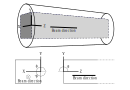
\includegraphics[width=\textwidth]{images/MicroBooNE/MicroBooNECoordinateSystem.pdf}
    \caption[MicroBooNE Coordinate System]{This image shows the MicroBooNE coordinate system. On top is a \gls{3d} overview of the \gls{tpc} active volume in the cryogenic vessel. At the bottom, from left to right, are the down stream view and the side view of the active volume. As can be seen, MicroBooNE uses a right handed coordinate system with the $x$-axis pointing against the drift direction, the $y$-axis pointing upwards, and the $z$-axis pointing in the direction of the neutrino beam. The angle $\phi$ is defined on the $x$-$y$-plane in the interval $\phi = [\SI{-180}{\degree},\SI{180}{\degree}]$, with $\phi = \SI{0}{\degree}$ being parallel to the $x$-axis and $\phi = \SI{90}{\degree}$ being parallel to the $y$-axis. Finally the angle $\theta$ is defined on the $y$-$z$-plane in the interval $\theta = [\SI{0}{\degree},\SI{180}{\degree}]$, with $\theta = \SI{0}{\degree}$ being parallel to the $z$-axis and $\theta = \SI{90}{\degree}$ being parallel to the $x$-$y$-plane. The coordinate system's origin $\vec{x}_0 = (0,0,0)$, is placed at the anode plane, on the half height point, at the upstream most part of the active volume.}
    \label{fig:MicroBooNECoordinateSystem}
\end{figure}
% TODO Make clear where the cathode and anode are in above picture ?

\subsection{High Voltage and Field Cage}
As established before, the \gls{tpc}'s drift motion is established in negative $x$-axis direction from cathode to the anode. For that purpose, a \gls{hv} feedthrough is employed to supply \SI{-70}{\kilo\volt} to the cathode. The design voltage was \SI{-128}{\kilo\volt}, but for reasons discussed in section \ref{sec:LArElectricField}, the collaboration never stood a chance to reach said voltage. The feedthrough is based on the ICARUS design \cite{ICARUST600}; a \SI{2.54}{\centi\metre} diameter inner conductor was inserted into the centre of a \SI{5.08}{\centi\metre} diameter hollow cylinder made of ultra-high molecular weight polyethylene. The upper part of this assembly was then pushed into an outer ground tube, completing the coaxial feedthrough assembly. The still visible polyethylene part was ripped in order to increase the surface distance from the conductor to the ground shield \cite{MicroBooNEDetector}. When inserted into the cryostat, the feedthrough makes contact with a receptacle cup mounted to the cathode, as shown in figure \ref{fig:HVFeedthrough}.
\begin{figure}[htbp]
    \centering
    \includegraphics[width=0.7\textwidth]{images/MicroBooNE/HVFeedthroughCryostat.jpg}
    \caption[HV Feedthrough of MicroBooNE]{This figure shows the \gls{hv} feedthrough after insertion into the cryostat \cite{MicroBooNEDetector}. The tip of the feedthrough rests in the cathode's receptacle cup and above the ripped polyethylene can be seen.}
    \label{fig:HVFeedthrough}
\end{figure}

MicroBooNE's field cage provides an uniform electric drift field of $E_0 = \SI{273.4}{\volt\per\centi\metre}$ (design: \SI{500}{\volt\per\centi\metre}), by means of an adapted voltage divider exhibiting three different stage circuits, see figure \ref{fig:VoltageDividerCircuits}. Under normal operations, all three exhibit a total resistance of \SI{250}{\mega\ohm}. Constituting the field cage are the aforementioned \num{64} field cage loops. The standard loops are numbered from \num{1} at the cathode to \num{64} at the anode. However, the cathode is also called loop \num{0}, since it is framed by a larger \SI{5.08}{\centi\metre} diameter tube.
\begin{figure}[htbp]
    \centering
    \subfloat[Field Cage Loops 0 through 16][Loops \num{0} through \num{16}]
    {
        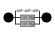
\includegraphics[width=0.32\textwidth]{images/MicroBooNE/VoltageDividerStageHigh.pdf}
        \label{fig:VDStageHigh}
    }
    \subfloat[Field Cage Loops 16 through 32][Loops \num{16} through \num{32}]
    {
        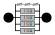
\includegraphics[width=0.32\textwidth]{images/MicroBooNE/VoltageDividerStageMid.pdf}
        \label{fig:VDStageMid}
    }
    \subfloat[Field Cage Loops 32 through 64][Loops \num{32} through \num{64}]
    {
        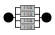
\includegraphics[width=0.32\textwidth]{images/MicroBooNE/VoltageDividerStageLow.pdf}
        \label{fig:VDStageLow}
    }
    \caption[MicroBooNE's Voltage Divider Circuits]{This figure shows the three different circuit diagrams of a MicroBooNE voltage divider stage. The black circles signify the field cage loops. In the higher voltage part \subref{fig:VDStageHigh}, from the cathode through loop \num{16}, uses two parallel Metallux HDR 969.23 resistors protected by three Panasonic ERZ-V14D182 varistors in series. The medium voltage part \subref{fig:VDStageMid}, from loop \num{16} through \num{32}, uses four parallel Ohmite Slim-Mox 104E resistors which are also protected by the aforementioned varistors. Finally, the lower voltage part \subref{fig:VDStageLow}, from loop \num{32} through \num{64}, features an unprotected Slim-Mox circuit.}
    \label{fig:VoltageDividerCircuits}
\end{figure}
The original design of MicroBooNE's field cage employed a simple voltage divider design, featuring four parallel Ohmite Slim-Mox 104E \SI{1}{\giga\ohm} resistors at each stage, as shown in figure \ref{fig:VDStageLow}. These are rated at \SI{1.5}{\watt} for a maximum voltage of \SI{10}{\kilo\volt} in air, which would be sufficient for normal operations with a design voltage of \SI{2}{\kilo\volt} across each resistor. In a cathode discharge event, however, these resistors could be stressed with peak voltage of up to \SI{80}{\kilo\volt} within a time frame of a few seconds \cite{MicroBooNEDetector}. This would undoubtedly destroy the Slim-Mox and thus render the \gls{tpc} defective. In fact, measurements showed their destruction already at voltages of \SI{32}{\kilo\volt}. Hence, the voltage divider circuit was adapted accordingly. In a first step the loops \num{0} through \num{32} where equipped with a surge protection circuit parallel to the resistors. The idea being that said protection circuit will be almost non-conductive with a resistance of the order of \SI{1}{\tera\ohm} during regular operations. But as soon as a voltage surge occurs, its resistance drops to orders of \SI{1}{\mega\ohm}, thus becoming conductive and carry the brunt of the currents developing in such an event \cite{SurgeProtection}. MicroBooNE's surge protection circuit consists of three Panasonic ERZ-V14D182 varistors in series, see figures \ref{fig:VDStageHigh} and \ref{fig:VDStageMid}, with individual clamping voltages of \SI{1.7}{\kilo\volt} at room temperature. Varistors are essentially diodes without a designated directionality, \ie they feature the same characteristic curve in both directions. The clamping voltage is in essence the threshold voltage at which the varistor becomes conductive. As these varistors are connected in series, the expected total clamping voltage amounts to $3\times\SI{1.7}{\kilo\volt} = \SI{5.1}{\kilo\volt}$. In the case of MicroBooNE, it was measured slightly higher at \SI{5.26(4)}{\kilo\volt} \cite{SurgeProtection}. In addition to the surge protection measures, loops \num{0} through \num{16} were connected with two, much more robust \SI{499}{\mega\ohm} Metallux HDR 969.23 resistors mounted in parallel, as shown in figure \ref{fig:VDStageHigh}. These feature a rating of \SI{23}{\watt} and \SI{48}{\kilo\volt} in air. Moreover, their failure mode is nondestructive, \ie if their voltage rating is exceeded, a breakdown occurs across the glass surface of the resistor. Thus their rating is limited by their surrounding medium and since \gls{lar} is an excellent insulator, they would be able to handle a peak voltage of \SI{80}{\kilo\volt} on their own with ease. Note, that every parallel set of resistors of the voltage divider features a total resistance of \SI{250}{\mega\ohm}. For the Metallux resistors \gls{fnal} engineering proposed a complicated and rather rigid mounting scheme using plastic insulator tubes and thick cables. This prompted M. Weber and myself to propose a much simpler, diagonal mounting scheme. For this, we designed flexible copper retainers allowing to reduce the stresses introduced by thermal contraction. The voltage divider mounting scheme is shown in figure \ref{fig:VoltageDividerPhotos}. The varistors and Slim-Mox resistors are both soldered onto a \gls{pcb}, which connects two adjacent field cage loops. The \gls{hv} and field cage design parameters are listed in table \ref{tab:FieldCageDimensions}.
\begin{figure}[htbp]
    \centering
    \subfloat[Voltage Divider Mounting Scheme][Voltage divider mounting scheme]
    {
        \includegraphics[width=0.48\textwidth]{images/MicroBooNE/VoltageDividerMetallux.jpg}
        \label{fig:VDMounting}
    }
    \subfloat[Surge protection varistors][Surge protection varistors]
    {
        \includegraphics[width=0.48\textwidth]{images/MicroBooNE/VoltageDividerVaristors.jpg}
        \label{fig:VDVaristors}
    }
    \caption[Pictures of MicroBooNE's Voltage Divider]{Picture \subref{fig:VDMounting} shows the mounting scheme of the MicroBooNE voltage divider inside the \gls{tpc}. It shows the first \num{16} loops being interconnected by the Metallux resistors fixed to the copper retainers designed by M. Weber and myself. On the top left side, the much smaller Slim-Mox (blue) resistors are shown. Picture \subref{fig:VDVaristors} shows the surge protection circuit with the three varistors (black) connected in series on a yellow \gls{pcb}. Both photographs are sourced from \cite{MicroBooNEDetector}.}
    \label{fig:VoltageDividerPhotos}
\end{figure}
\begin{table}[hbtp]
    \centering
    \caption[MicroBooNE's Field Cage and HV Design Parameters]{MicroBooNE's field cage and \gls{hv} design parameters.}
    \begin{tabu} to 0.7\textwidth{lrl} \toprule
    Parameter & Value & Unit \\ \midrule
        Field cage width ($x$-axis) & \num{2.560} & \si{\metre} \\
        Field cage height ($y$-axis) & \num{2.325} & \si{\metre} \\
        Field cage length ($z$-axis) & \num{10.368} & \si{\metre} \\
        \Gls{lartpc} active volume & \num{61.71} & \si{\metre\cubed} \\
        \Gls{lartpc} active mass (at standard \gls{bp}) & \num{86.15} & \si{\tonne} \\
        Number of field-cage loops & 64 & \\
        Design cathode voltage & \num{-128} & \si{\kilo\volt} \\
        Operation cathode voltage & \num{-70} & \si{\kilo\volt} \\
        Design Drift field strength $\vec{E}$ & \num{500} & \si{\volt\per\centi\metre} \\
        Operation Drift field strength $\vec{E}$ & \num{273.4} & \si{\volt\per\centi\metre} \\
        Design loop to loop potential & \num{2.0} & \si{\kilo\volt} \\
        Operation loop to loop potential & \num{1.09} & \si{\kilo\volt} \\ \bottomrule
    \end{tabu}
    \label{tab:FieldCageDimensions}
\end{table}
% TODO add full drift time: design and operation 

In my view, the choice of varistors for surge protection was quite risky, as they use to fail short. We also observed cracking at their surfaces after a single cooling cycle. This can be attributed to their ceramic nature. It would have been safer to only install the large Metallux resistors between the loops \num{0} and \num{32}, for they proved to be reliable. Alternatively, the use of gas discharge tubes instead of varistors would have been a low-risk option as well \cite{SurgeProtection}. The latter were dismissed, because it was feared they could contaminate the \gls{lar} with nitrogen in case of a failure. I personally find this fear unfounded, since other than the varistors, none of these discharge tube failed during testing. Anyhow, it has to be added, that at the time of detector construction, the Metallux resistors where only available in limited quantities. Waiting for more to be produced undoubtedly would have delayed the experiment.  

\subsection{Charge Readout Planes}
MicroBooNE's charge readout consists of three wire planes, two planes run in induction mode (U- and V-plane) and one in collection mode (Y-plane). As the name implies, the Y-wires orientation is vertical and therefore parallel to the $y$-axis, \ie in \SI{90}{\degree} angle to the $z$-axis. Since the orientation of each wire plane is rotated by \SI{60}{\degree}, the angles of the U-plane and V-plane wires with respect to the $z$-axis are \SI{30}{\degree} and \SI{-30}{\degree}, respectively. A picture of the MicroBooNE readout wires is shown in figure \ref{fig:WirePlaneSetup}. \begin{figure}[htbp]
    \centering
    \includegraphics[width=0.9\textwidth]{images/MicroBooNE/WirePlaneSetup.pdf}
    \caption[Wire Plane Configuration of MicroBooNE]{This picture shows the wire plane configuration of the MicroBooNE \gls{tpc}. A single wire of every plane is colourised: U-plane in green, V-plane in blue, and Y-plane in red. Furthermore, the angles with respect to the horizontal $z$-axis are given for these representative wires. This closeup photograph was taken from the inside of the \gls{tpc} and thus the reference system for the wire angles are mirrored. It is in fact the view from a \gls{quasifreeelectron} approaching the readout planes.}
    \label{fig:WirePlaneSetup}
\end{figure}
Each plane exhibits a \SI{3}{\milli\metre} spacing to its respective neighbouring plane. Also, the wire pitch of neighbouring wires within each plane amounts to \SI{3}{\milli\metre}. Both \glspl{InductionPlane} features \num{2400} wires each, while the \gls{CollectionPlane} consists of \num{3456} wires, resulting in a total of \num{8256} charge readout channels. These wires are all made of stainless steel and measure \SI{150}{\micro\metre} in diameter. Moreover, they are coated with a \SI{2}{\micro\metre} layer of copper topped with \SI{0.1}{\micro\metre} of silver, insuring increased charge collection capabilities. They are tensioned with a force of \SI{6.9(10)}{\newton}. Drifting \glspl{quasifreeelectron} arriving at the readout will first drift through the U-plane and later the V-plane producing an induction signal, as discussed in section \ref{sec:ChargeReadout}, figure \ref{fig:WireSignals}. Finally, the charge carriers will be collected at the Y-Plane leaving a typical collection signal also shown in figure \ref{fig:WireSignals}. In order to achieve the \gls{InductionPlane} transparency the U-wires are biased with \SI{-200}{\volt}, the V-wires are at ground potential, and the Y-wires have \SI{400}{\volt} applied. The aforementioned design parameters of the charge readout planes are summarised in table \ref{tab:ReadoutWireParameters}.
\begin{table}[hbtp]
    \centering
    \caption[MicroBooNE's Wire Planes Design Parameters]{MicroBooNE's wire planes design parameters.}
    \begin{tabu} to 0.7\textwidth{lrl} \toprule
        Parameter & Value & Unit \\ \midrule
        Number of anode planes & \num{3} & \\
        Anode plane spacing & \num{3} & \si{\milli\metre} \\
        Wire pitch within plane & \num{3} & \si{\milli\metre} \\
        Wire diameter (including coating) & \num{154.2} & \si{\micro\metre} \\
        Design wire tension & \num{7} & \si{\newton} \\
        Achieved wire tension & \num{6.9(10)} & \si{\newton} \\
        Total number of wires & \num{8256} & \\
        Number of wires in U-plane & \num{2400} & \\
        Number of wires in V-plane & \num{2400} & \\
        Number of wires in Y-plane & \num{3456} & \\
        U-plane wire angle w.r.t. $z$-axis & $+\num{30}$ & \si{\degree} \\
        V-plane wire angle w.r.t. $z$-axis & \num{-30} & \si{\degree} \\
        Y-plane wire angle w.r.t. $z$-axis  & \num{90} & \si{\degree} \\
        U-plane bias voltage & \num{-200} & \si{\volt} \\
        V-plane bias voltage & \num{0} & \si{\volt} \\
        Y-plane bias voltage & \num{400} & \si{\volt} \\
        U- to V-plane gap electric field & \num{666.7} & \si{\volt\per\centi\metre} \\
        V- to Y-plane gap electric field & \num{1466.7} & \si{\volt\per\centi\metre} \\
        \bottomrule
    \end{tabu}
    \label{tab:ReadoutWireParameters}
\end{table}

For installation purposes, each individual wire is wrapped around a brass ferrule and twisted at both of its ends. The ferrules of several wires are then placed between two \glspl{pcb} and sealed in by two press-fit rivets, forming wire carrier boards. At one side each wire is weaved around two pins in the carrier board which are connected to a readout connector on the top side of the board. Said boards carry groups of 16 induction, or 32 collection wires, respectively. The above-described wire carrier board assembly is depicted in figure \ref{fig:WireCarrier} below.
\begin{figure}[htbp]
    \centering
    \subfloat[Wire Ferrule][Wire ferrule with twisted wire]
    {
        \includegraphics[width=0.48\textwidth]{images/MicroBooNE/WireTwist.pdf}
        \label{fig:WireTwist}
    }
    \subfloat[Wire Carrier Board][Wire carrier board]
    {
        \includegraphics[width=0.48\textwidth]{images/MicroBooNE/WireCarrierBoard.png}
        \label{fig:WireCarrierBoard}
    }
    \caption[MicroBooNE's Readout Wire Carrier]{Above pictures show the wire carrier board assembly \cite{MicroBooNEDetector}.}
    \label{fig:WireCarrier}
\end{figure}
These wire carrier boards are then secured between studs welded onto stainless steel tensioning bars. In order to achieve equally spaced planes, the carrier boards of the three different planes are stacked on top of each other. The tensioning bars are then embedded in the C-shaped anode frame structure, where they are adjusted and secured by a set of bronze screws ensuring a more or less uniform tension of \SI{6.9(10)}{\newton}.

The wire plane structure of MicroBooNE proved to leave room for improvement. Proper tensioning while still ensuring the correct wire position was very challenging. This might also be underpinned by the large amount of dead readout channels, as I suspect several of the long wires to be touching others from different planes. Some of these dead channels can also be attributed to mistakes made during the assembly process, see section \ref{sec:MicroBooNELessonsLearned}. In total about \SI{30}{\percent} of the wire plane area is covered by at least one dead channel. Just about \SI{3}{\percent} of the total area feature more than one dead channel, and hence, are unsuitable for particle track reconstruction \cite{MicroBooNEDeadWires}. This dead wire situation in MicroBooNE is depicted in figure \ref{fig:DeadWires}.
\begin{figure}[htbp]
    \centering
    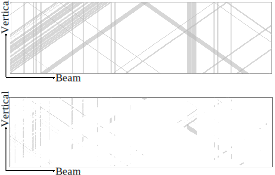
\includegraphics[width=0.9\textwidth]{images/MicroBooNE/DeadWires.pdf}
    \caption[Dead Wires of MicroBooNE]{In the top figure, all dead readout wire channels are sown in grey. The bottom graph shows the readout area unsuitable for reconstruction, where the signal of at least two wire planes is missing. About \SI{30}{\percent} of the area, has at least one channel missing and around \SI{3}{\percent} of the area is dead \cite{MicroBooNEDeadWires}. This figure is sourced from \cite{MicroBooNEDeadWires}.}
    \label{fig:DeadWires}
\end{figure}
The issue of touching wires could be resolved by plastic spacers similar to the ones used in the ICARUS T600 detector \cite{ICARUST600}. They installed small plastic pegs at each vertical wire frame pillar. These feature three grooves with a \SI{3}{\milli\metre} spacing for the wires to be inserted. The pegs then hold the wires in their intended position.

\subsection{Light Detection System} \label{sec:MicroBooNELightDetection}
MicroBooNE features two different light detection systems. The primary system consists of \num{32} optical units, while the secondary system comprises four light guide paddle prototypes. The paddles of the secondary light detection system are each made of six \gls{tpb} coated acrylic light guide bars. At the light readout end of the paddles, said bars are twisted, stacked together, and optically connected to a \num{2} inch Hamamatsu R7725-MOD \gls{pmt}. Officially these paddles are a R\&D project, however, the choice of \glspl{pmt} as light detectors already seemed to be outdated at the time of conception in view of \glspl{sipm} based systems I discussed in section \ref{sec:LightReadoutSystems}. Both, the \gls{tpb} coating as well as the \gls{pmt} of the secondary system exhibit lower photon efficiencies than the primary system. In order to mitigate this, the active surface area of the paddle is larger \cite{MicroBooNEDetector}.

The optical units of the primary system, on the other hand, are a conservative solution by choice \cite{MicroBooNEProposal1,MicroBooNEProposal2} and are based on the ICARUS design \cite{ICARUST600}. One optical unit consists of a Hamamatsu R5912-02MOD \num{8} inch \glspl{pmt}, seated $\sim\SI{3}{\milli\metre}$ behind a \gls{tpb} coated acrylic plate with a \SI{305}{\milli\metre} diameter. The side of the \gls{pmt} is covered by a mu-metal shield in order to protect the multiplier stages from the adverse influence of the earth's magnetic field. All these components are held in place by an elaborate mounting structure, forming the so-called \textbf{optical unit}, see figure \ref{fig:OpticalUnit}. The units are installed evenly in the $y$-$z$-plane \SI{12.7}{\centi\metre} behind the charge readout planes \cite{MicroBooNEDetector}, as shown in figure \ref{fig:LightDetectorsMounted}.
\begin{figure}[htbp]
    \centering
    \resizebox{\textwidth}{!}{
    \subfloat[Primary Optical Unit][Primary optical unit]
    {
        \includegraphics[height=5cm]{images/MicroBooNE/PMTAssemblyCAD.pdf}
        \label{fig:OpticalUnit}
    }
    \subfloat[Installed Optical Units][Installed optical units]
    {
        \includegraphics[height=5cm]{images/MicroBooNE/MicroBooNEInside2.jpg}
        \label{fig:LightDetectorsMounted}
    }
    }
    \caption[MicroBooNE's Light Detection System]{In \subref{fig:OpticalUnit} a primary unit of MicroBooNE's light detection system is shown \cite{MicroBooNEDetector}. Figure \subref{fig:LightDetectorsMounted} shows the assembled light detection system from inside the \gls{tpc} through the wire planes.}
    \label{fig:LightDetectionSystem}
\end{figure}
Now, if scintillation photons hit the optical units, their wavelength will first be shifted from \SI{128}{\nano\metre} to $\sim\SI{450}{\nano\metre}$ by the \gls{tpb} coating on the acrylic plates. From there, these photons are emitted in all directions and some of them eventualy hit the photocathode of the \glspl{pmt}, producing a photoelectron. Said electron is then amplified by the dynode cascade, which is described in more detail in section \ref{sec:LightReadoutSystems}. Note, that the secondary system follows the same principle, with the small difference that the wavelength shifted photons are guided by the light guide to the \gls{pmt}. 

The centrepiece of the light detection system, the Hamamatsu R5912-02MOD \gls{pmt}, features a photocathode diameter of \num{8} inches or \SI{202}{\milli\metre}, and a total of \num{14} dynode stages. At its optimal operating voltage of \SI{1700}{\volt}, the \gls{pmt} exhibits a staggering gain of \num{e9} at room temperature. However, around \SI{87}{\kelvin} said gain is reduced by \SIrange{10}{50}{\percent} for individual \glspl{pmt} \cite{MicroBooNEDetector}. Furthermore, the \gls{pmt} is optimised or modified for cryogenic applications, hence the affix ``02MOD'' in its designation. This modification comes in form of a thin platinum layer below the photocathode in order to ensure sufficient conductance at low temperatures. In MicroBooNE, these \glspl{pmt} are operated in reverse bias mode, see section \ref{sec:LightReadoutSystems}. This configuration has two major advantages: first, there is only one cable needed for every \gls{pmt}, and second, it minimises inadvertent electric fields between the photocathode and the \gls{CollectionPlane}. During operations, a single \gls{pmt} needs to provide a gain of \num{3e7} in \gls{lar}, wherefore the \gls{pmt} voltage is set at about \SI{1300}{\volt} with a spread between \SIlist{1185;1460}{\volt} on individual \glspl{pmt} \cite{MicroBooNEDetector}. This is done, because the scintillation light yield in \gls{lar} is so high, that the \gls{pmt} would saturate at higher gains and thus hamper accurate photon intensity measurements. The average quantum efficiency of the \gls{pmt} across the \gls{tpb} emission spectrum from \SIrange{400}{525}{\nano\metre}, amounts to \SI{15.3(8)}{\percent} \cite{MicroBooNEDetector}. This means, that \SI{15.3}{\percent} of the photons of said spectrum, incident to the photocathode, are registered as a signal. In addition, the expected yield of visible photons per incident \SI{128}{\nano\metre} photon of the \gls{tpb} coated acrylic plate is \num{0.98(17)} \cite{MicroBooNEDetector}. The quantum efficiency of the whole optical unit, however, is certainly well below \SI{10}{\percent}, for the geometry of the setup allows less than \SI{30}{\percent} of the \gls{tpb} emitted photons to reach the photocathode of the \gls{pmt}, although official numbers are not published.

In my view, the choice of \gls{pmt} type for MicroBooNE's primary light detection system is not ideal. The Hamamatsu R5912-02MOD is a high sensitivity device and is the third largest \gls{pmt} Hamamatsu builds. Obviously, it is conceived for low light yield experiments and not for \glspl{lartpc} the size of MicroBooNE's. I see this suspicion confirmed by the low operation voltage of \SI{1300}{\volt}. Operating such an expensive high gain \gls{pmt} at this low voltage is the equivalent of buying a Ferrari and driving it only up to the 3\textsuperscript{rd} gear. Personally, I would prefer a system with smaller \glspl{pmt}, and to compensate the smaller photocathode area, I would at least double the amount of optical units. This would increase the spacial resolution without compromising the overall sensitivity. Unfortunately, there seem no lessons learned from MicroBooNE on that front, since the next generation of neutrino detector, \gls{sbnd}, makes use of the same \glspl{pmt} for its primary optical system. This is doubly disappointing, because not only does the next generation use a conservative light detection system, but it also seems to repeat deficiencies of previous experiments. However, \gls{sbnd} also features a secondary system based on \glspl{sipm} \cite{SBNDLightReadoutSystem}. The secondary optical units will be deployed in the same quantity as the primary ones.

% TODO Maybe try to verfy the 67.5 % and the 10.3 %? Only god and me knew where these numbers are from, now only god knows!
% The wave length conversion efficiency of the plates is expected to be \SI{67.5(75)}{\percent} per incident \SI{128}{\nano\metre} photon. In the \gls{tpb} emission spectrum (\SIrange{400}{525}{\nano\metre}) the averaged \gls{pmt} quantum efficiency is found to be \SI{15.3(8)}{\percent} which leads to an overall spectrum-averaged quantum efficiency of a optical unit of \SI{10.3(13)}{\percent}. All the 32 optical units constitute the primary light collection system. 

\subsection{Signal Readout and Processing} \label{sec:MicroBooNEReadout}
To be able to analyse \gls{lartpc} data, the signals from the various detector systems need to be in a processable digital format. Hence, the analogue raw signals of the \num{8256} charge readout wires and the \num{36} \glspl{pmt} need to be amplified, digitised, and written to storage devices. The first step is realised using amplifiers and the latter two are performed by the so-called \gls{daq} system. This chain of signal processing in MicroBooNE is shown in figure \ref{fig:ReadoutSystem}.
\begin{figure}[htbp]
    \centering
    \includegraphics[width=1.0\textwidth]{images/MicroBooNE/DAQScheme.pdf}
    \caption[Schematics of the MicroBooNE Signal Readout System]{Depicted above is a schematic representation of MicroBooNE's signal readout system for the \gls{tpc} and the \glspl{pmt}. On the left side, the cryostat is shown, where the analogue signals are generated and amplified. On the right, the \gls{daq} system is depicted, which is responsible for digitisation and writing the data to storage. This figure is sourced from \cite{MicroBooNEDetector}.}
    \label{fig:ReadoutSystem}
\end{figure}
% TODO change the PMT count on this figure, it is 36 not 30!

By far the weakest raw signals in a \gls{lartpc} stem from the charge readout wires. As discussed in section \ref{sec:ChargeReadout}, a single collection wire only provides a signal strength of the order of \SI{1}{\femto\coulomb}. Such signals are too weak to be directly digitised, and thus, the signals need to be amplified first. For this purpose, a novel cryogenic analogue front-end \gls{asic} was designed for MicroBooNE. Said \gls{asic} is based on a \SI{180}{\nano\metre} \gls{Photolithography} process and consist of about \num{15000} transistors. It integrates the preamplifiers and signal shapers for \num{16} channels on a single chip. Furthermore, it features an input shift register facilitating programmable settings for gain (\SIlist{4.7;7.8;14;25}{\milli\volt\per\femto\coulomb}), peaking time (\SIlist{0.5;1.0;2.0;3.0}{\micro\second}), as well as voltage baseline (\SIlist{200;900}{\milli\volt}) \cite{LArASIC1}. The last-mentioned setting allows for the use of the same chip for collection and induction wires, \ie for unipolar and bipolar signal as shown in figure \ref{fig:WireSignals}. Most importantly, this \gls{asic} shows the same amplification and shaping properties in \gls{lar} and at room temperature \cite{LArASIC2}. Naturally, the thermal noise level is greatly reduced in cryogenic environments. A further advantage of the cryogenic front-end electronics is posed by the close proximity of the amplification to the signal's origin, which also reduces noise. Moreover, the \gls{asic} only produces a heat output of $\sim\SI{6}{\milli\watt}$ per channel. MicroBooNE employs a total \num{516} \glspl{asic} with a total heat output of $\sim\SI{50}{\watt}$, which can be handled by the cryogenic system with ease. The \glspl{asic} are mounted on a \glspl{pcb}, which directly connects to three wire carrier board stacks. Hence, \num{12} \glspl{asic} are needed to host these \num{192} readout channels ($\num{3}\times\num{32}$ collection, and $\num{2}\times\num{3}\times\num{16}$ induction channels). A picture of such a \gls{pcb} is shown in figure \ref{fig:ReadoutBoard}.
\begin{figure}[htbp]
    \centering
    \includegraphics[width=1.0\textwidth]{images/MicroBooNE/ReadoutBoard.pdf}
    \caption[Front-End Electronics PCB]{Shown here is MicroBooNE's front-end electronics \gls{pcb}. The board features \num{12} front-end \glspl{asic} (six on each side) and a total \num{192} readout channels. The three wire carrier board input connectors are mounted on the top on the other side of the board. The bottom output connectors are used to carry the amplified signal to the \gls{daq} system. Finally, the connectors on the sides provide board power and shift register inputs and outputs. This picture is sourced from \cite{LArASIC2}.}
    \label{fig:ReadoutBoard}
\end{figure}
The \gls{asic} settings are adjusted by a shift register, wherefore they can be daisy-chained. This has the advantage, that less cables are needed, however, if one of the shift registers fails, the whole chain after the defective \gls{asic} might not be programmable anymore. Still, the development of these \gls{asic} based front-end electronics mark a breakthrough in the \gls{lartpc} field. For instance, our group at the \gls{lhep} measured a massive improvement of the signal-to-noise ratio by a factor of \num{6} compared to conventional preamplifiers in Argontube \cite{LArASICTestArgontube}.

Once amplified, the signal is transmitted via twisted-pair cabling of $\sim\SI{2.5}{\metre}$ length to the signal feedthroughs, where it gets extracted from the \gls{lar} environment. At every feedthrough, intermediate amplifiers with a gain of $\sim\SI{12}{\decibel}$ ensures a smooth transmission by $\sim\SI{20}{\metre}$ long shielded twisted pair cables to the \gls{daq} system\cite{MicroBooNEDetector}. Above-described signal transmission is also depicted in figure \ref{fig:ReadoutSystem}.

As mentioned above, the \gls{daq} system serves two purposes: digitisation, and data storage. The first step is handled by a total of \num{1040} Analog Devices AD9222 \glspl{adc} \cite{ADCDataSheet}. Each \gls{adc} chip digitises the signal of \num{8} charge readout channels and features a peak-to-peak differential range of \SI{2}{\volt} with resolution of \num{12} bits, \ie a voltage resolution of \SI{0.488}{\milli\volt}. For MicroBooNE, the \gls{adc}'s sampling rate was chosen to be \SI{16}{\mega\hertz}. The \glspl{adc} themselves are grouped into modules of \num{8} on a single \gls{pcb}, which are controlled by a so-called \gls{fem}. Thus, there are \num{130} \gls{adc} modules and \glspl{fem}, handling \num{64} channels each. The centrepiece of a \gls{fem} is a Stratix III \gls{fpga} manufactured by Altera. It handles the whole data stream originating from the respective module. In the \gls{fem} the data rate is reduced to \SI{2}{\mega\hertz}, since a typical wire signal width is of the order of \SI{1}{\micro\second} due to charge carrier diffusion, as discussed in section \ref{sec:ChargeDrift}. The \gls{fpga} then writes the data from all \num{64} channels sequentially into a \gls{sram} based \gls{RingBuffer}. Once a trigger signal arrives, the data is the \gls{fpga} reads the data back from memory, performs a lossless Huffman compression, and send it to a transmitter module. The latter then transfers the data to computers, where it is written to storage, see \ref{fig:ReadoutSystem}. There is actually a second, constant data stream used for supernova neutrino studies, but I will not describe it in detail here, as it does not pertain to the topic of this thesis.

The \gls{pmt} raw signal is guided through the \gls{hv} coaxial cable and a feedthrough out of the cryostat, where a splitter circuit decouples the signal from the \gls{hv} source by an AC-coupling capacitor. Thereafter the signal gets split, this time through different resistor chains, into a high-gain (attenuation factor \num{0.18}), and a low-gain (attenuation factor \num{0.018}) channel. Both, high-gain and low-gain channels, are split again thereafter creating four channels from a single \gls{pmt} signal ($\num{32} \times \num{2} \times \num{2}$). This procedure allows for a wide dynamic signal range at the \gls{adc} readout stage. Thereafter, the raw signals run through a shaping amplifier, which converts them into an unipolar signal with a \SI{60}{\nano\second} rise time before digitisation. The \gls{adc} used for the \gls{pmt} readout is the Texas Instruments ADS5272 \cite{ADCPMTDataSheet}. Like the wire channel \gls{adc}, it too features \num{8} channels in a single chip, a range of \SI{2}{\volt}, and a \num{12} bit resolution. The sampling rate, however, is four times higher at \SI{64}{\mega\hertz}. This design choice arises from the fact that the \gls{pmt} signals are much shorter, \ie \SI{60}{\nano\second} versus \SI{1}{\micro\second} rise time. Note, that all \glspl{adc} of the \gls{daq} system are synchronised by an external clock of \SI{16}{\mega\hertz}. In the case of the \gls{pmt} readout this clock frequency is multiplied by a factor of four. Six light readout \gls{adc} chips are grouped together in a single module for the digitisation of \num{48} differentially-driven channels. Every module is controlled by an \gls{fem} as well. Hence, there are three modules hosting the whole of both light readout system channels. The light readout \gls{fem} functions similarly to the wire readout \gls{fem}, however, there are three key differences: First, the clock frequency is not reduced, second, a zero-suppression is performed instead of a Huffman compression, and third, the \gls{fpga} also acts as a \gls{Discriminator} to produce the \gls{pmt} trigger signal. There are three criteria for the \gls{pmt} trigger: There must be more than one \gls{pmt} firing and a combined pulse height of at least two \gls{pe}, all within a \SI{100}{\nano\second} time window. During \gls{bnb} measurements, said trigger needs to coincide with the \SI{1.6}{\micro\second} \gls{BeamGate} trigger. These combined trigger signals are then distributed to the \glspl{fem} of all digitisation modules, in order to write the event data. The digitised \gls{pmt} signals are recorded in two different modes: either in a continuous, unbiased readout window of \SI{23.4}{\micro\second} which is opened by the \gls{BeamGate} signal, or in discriminated pulses (referred to as cosmic-discriminator) each in a window of $\sim \SI{1}{\micro\second}$. The latter mode is activated if, for any given tube, the \gls{adc} count goes above a \num{80} \gls{adc} counts (roughly \num{4} \gls{pe}), \ie the \glspl{pmt} are essentially self-triggering their data recording. These two different formats are saved in an event as output waveforms. In \gls{lartpc} jargon, a scintillation event recorded by a single \gls{pmt} is named \gls{OpticalHit} and a collection of any correlated \glspl{OpticalHit} is called a \gls{Flash}.

\subsection{Lessons Learned during Detector Assembly} \label{sec:MicroBooNELessonsLearned}
For me personally, MicroBooNE was not the first \gls{lartpc} I encountered in my career. During my master's thesis research at the \gls{lhep} of the University of Bern in 2011 and 2012, I became a part of the ARGONTUBE group. At this time, the group was very active and I was involved in the conception, construction and operation of three different \gls{lartpc} prototypes as well as the ARGONTUBE detector itself. As a part of a rather small group I gained expertise in all subsystems of a \gls{lartpc} experiments, from cryogenics to readout electronics. In the following years, as a PhD student, I was further involved in more ARGONTUBE runs and various test setups, \ia investigating \gls{pmt} induced wire noise, \gls{lcs} prototyping, and \gls{hv} discharge measurements. The day I visited \gls{fnal} for the first time and joined the collaboration, I became a member of the MicroBooNE detector assembly team. Thenceforth, I have been involved in almost every single step of \gls{tpc} construction. Thus, I gained insights in many issues, organisational and hardware related, which I would like to share here in the form of a personal lessons learned. This is in no way meant as a finger-pointing exercise, but as factual and constructive criticism based on my experience with the \gls{lartpc} technology. Moreover, it has to be noted that MicroBooNE is the only \gls{lartpc} based experiment which was operational for a period of five consecutive years. No other experiment reached this level of operational stability so far.

A general issue was the task scheduling. Most of the time, ambitious deadlines were set and thus we were always in a hurry to finish the task at hand. Usually, after finishing said task, we found out that \gls{tpc} construction was halted because of missing parts, changes in design, or engineering problems. Often the work on the detector was interrupted for several months, all while the ambitious schedule got stretched out further. Once the issues were resolved, we again had to aim for the next ambitious deadline. This did not make sense in my view. Although it looked bulky, we were actually building a sensitive scientific instrument. Rushing the construction only to let it accumulate dust for a longer time is not ideal. 

Another issue was introduced by the contracted manufacturers. They often did not deliver their parts in compliance with specifications. It all started with the field cage tubes. Six of these tubes with various length represent the main components of a single field cage loop. These tubes were ordered in clean and deburred condition, but they arrived covered in grease and had metal shards in almost every drill hole. Yet, they were not returned to the manufacturer, because of the collaboration's tight assembly schedule. So, we deburred and cleaned almost \num{400} tubes. During this process, it became obvious that all of the tubes showed a great variation in length, often several centimetre. For a detector with a targeted tolerance value of \SI{1}{\milli\metre}, this did not bode well. However, this would not influence the drift field uniformity significantly, as long as the loops are properly spaced. The manufacturing quality problems did not stop there. Most notably, the C-shaped girders of the anode frame did not arrive in that shape and had to be rigged with pulleys and hydraulic jacks to fit their purpose. In hindsight, it would have been better to return these parts, as we could not hold on to the schedule anyway. In my view, with regular visits to the manufacturers these issues could have been identified early and ensured an increased level of quality.

There were also a great number of engineering inconsistencies I observed. For example, there were wire tensioning screw holes planned to go through two adjacent pieces of metal. Obviously, the threads did not match and we were not able to tension the wire bar at these positions. This could have been avoided, if one of the metal plates featured a through hole instead of a threaded one. Another issue arose when assembling the cathode frame. This is a trussed structure made of hollow sections made of stainless steel, see figure \ref{fig:MicroBooNETPCCathode}. Since the sections had to be bolted together in \SI{45}{\degree} angles, there were metal plates with threads welded to the hollow sections in a \SI{45}{\degree} angle. Although the welds were well done and the structure was assembled on a flat surface, we were not able to mount the frame within the \SI{1}{\milli\metre} tolerance. Just welding is definitively not the right manufacturing method for these parts. Moreover, there where the cathode sheets, made of stainless steel, which featured far too few suspension points. The few suspension points present did often not fit the warped cathode frame and had to be enlarged with a Dremel. Thus, the cathode sheets buckled and had to be TIG-welded to the cathode frame where possible. All these circumstances led to a \SIrange{-6.498}{6.636}{\milli\metre} deviation from a flat cathode \cite{MicroBooNEDetector}, as shown in figure \ref{fig:CathodeWarp}.
\begin{figure}
    \centering
    \subfloat[Cathode Warp Left][]
    {
        \includegraphics[width=0.48\textwidth]{images/MicroBooNE/CathodeWarpLeft.jpg}
        \label{fig:CathodeWarpLeft}
    }
    \subfloat[Cathode Warp Right][]
    {
        \includegraphics[width=0.48\textwidth]{images/MicroBooNE/CathodeWarpRight.jpg}
        \label{fig:CathodeWarpRight}
    }
    \caption[MicroBooNE's Cathode Warp]{These two figures show the cathode warp, \ie deviation from flat, as measured by a survey. The deviations measure from \SI{-6.498}{\milli\metre} (red) to \SI{6.636} (blue). These figures are sourced from \cite{MicroBooNEDetector}.}
    \label{fig:CathodeWarp}
\end{figure}
Finally, there were several parts whose design was never finalised, yet they were ordered in their unfinished state. Chief among these, are the cathode tubes which constitute field cage loop \num{0}. In their design state, they interfered with the cathode sheets, and did not attach to neither the cathode frame, nor to other cathode tubes to form a loop. Too me it seemed, as if there was no engineering review process in place to catch these mistakes.

Then there were several design issues, which I already covered in the various sections above. Prime among these, was the aforementioned field cage resistor choice, which ended in the implementation of a variety of different field cage circuits. Actually, this was the last issue delaying the detector completion by several months and the pressure to just finish the construction of the \gls{tpc} was high. I dare say, that a lot of the decisions made concerning surge protection were influenced by emotions rather than levelheadedness. Luckily, the field cage worked, despite the, in my opinion, risky choice of varistors. Also the wire tensioning and dead channel issues partially fall into the category of design flaws. We considered testing the proper wire spacing by applying the bias voltage to the planes in order to identify touching wires before inserting the \gls{tpc} into the cryostat. Regrettably, this idea was discarded because of safety concerns about open \gls{hv} sources. I still think this test could have been performed safely from a distance, using designated electronics, but it would have delayed the construction even further.

Finally, there were also construction errors. Most of them were of minor relevance or corrected. Yet there was one mistake, that should not have passed quality control. One of the front-end electronics boards, shown in figure \ref{fig:ReadoutBoard}, was only plugged into one row of wire carrier board pins, shown in figure \ref{fig:WireCarrierBoard}. Hence, a block of \num{96} neighbouring collection wires was neither instrumented nor connected to the bias voltage, \ie these channels are dead. Wire readout tests, which showed abnormally low noise levels for these channels, were simply ignored.

\section{Cosmic-Ray Tagger} \label{sec:CRT}
The latest addition to MicroBooNE is the \gls{crt}. The reason for its existence is the large amount of cosmic background pileup prevalent in the MicroBooNE \gls{tpc}, a phenomenon discussed in section \ref{sec:CosmicPileup}. Said pileup is able to contribute significantly to the background of the \gls{lee} studies, as I will show in a small cosmic background simulation in chapter \ref{sec:CosmicRayGammaBackground}. Likewise, cross section measurements are affected by said pileup. For instance, MicroBooNE is exposed to a cosmic-ray muon rate of \SI{5.5}{\kilo\hertz}, which leads to around \num{13} particle traces to be visible within the \SI{2.25}{\milli\second} readout window \cite{MicroBooNEMuonRate}. It is merely impossible to identify the $t_0$ of each background event by means of \gls{Flash}-matching, using MicroBooNE's light detection system \cite{MicroBooNEFlashMatching}. Hence, our team at \gls{lhep} conceived the \gls{crt} to be used in all \gls{sbn} experiments \cite{CRTGeneral}. The general idea is, to clad the \gls{lartpc} in plastic scintillator detectors. These detectors need to be position sensitive to $\mathcal{O}(\SI{1}{\centi\metre})$ and time sensitive to $\mathcal{O}(\SI{100}{\nano\second})$, in order to tag tracks in the \gls{tpc} readout stream with the \gls{crt} signals. MicroBooNE's \gls{crt} system is shown in figure \ref{fig:CRTInstallation}. As can be seen, the cryostat is not completely wrapped by scintillator panels, because of spacial constraints and since the \gls{crt} was an unplanned addition to MicroBooNE. Still, the compact design of the \gls{crt}, mostly due to the use of \glspl{sipm}, made it possible to add it as a additional detector system in the first place. It should also be mentioned, that I will only touch briefly on the \gls{crt} topic. For an in-depth discussion of the \gls{crt}, the PhD thesis of T. Mettler \cite{CRTThomasPhD} and our paper on the matter \cite{CRTGeneral} should be consulted.
\begin{figure}[htbp]
    \centering
    \includegraphics[width=0.8\textwidth]{images/MicroBooNE/CRTInstallationCAD.png}
    \caption[3D Rendering of MicroBooNE's CRT]{This figure depicts a \gls{3d} rendering of MicroBooNE's \gls{crt}. In the picture the cryostat in the middle and the electronics racks on top of the platform are made transparent for better view of the system. This picture is sourced from T. Mettler's thesis \cite{CRTThomasPhD}.}
    \label{fig:CRTInstallation}
\end{figure}

\subsection{Scintillator Module}
The \gls{crt} is composed of modules containing \num{16} plastic scintillator strips placed side by side, each featuring a width of \SI{10.8}{\centi\metre} and a thickness of \SI{1}{\centi\metre}, see figure \ref{fig:CRTModule}. The respective module length is variable, from \SIrange{1.3}{4.1}{\metre}, depending on the module's position. For MicroBooNE's \gls{crt} a total of \num{73} modules were installed \cite{MicroBooNECRT}. The scintillation material used is a USMS-03 polystyrene-based mixture, with an emission maximum around \SI{430}{\nano\metre}, produced by UNIPLAST. The surface of the strips is subjected to a structural treatment, resulting in the formation of a highly reflective white layer \cite{CRTGeneral}. On both sides of the strips, a \gls{wls} fibre is glued into a groove, ranging over the whole strip length. The fibre is made by Kuraray (type: Y-11(200), diameter: \SI{1}{\milli\metre}) and features an absorption peak at \SI{430}{\nano\metre}, while its emission peak is located around \SI{476}{\nano\metre} \cite{CRTFibreSpecs}. Note, that the fibre is not primarily required for \gls{wls}, but as a high efficiency light guides. The \glspl{sipm} used as detectors would also function with \SI{430}{\nano\metre}, however, to bundle the light onto them is best achieved by these fibres. The groove containing the fibre is covered by a reflective Mylar tape in order to reduce photon losses. On the readout end, every fibre is optically coupled to a \gls{sipm}. The other end of the fibre is aluminium coated to increase photon yield further by reflection. As \gls{sipm}, the Hamamatsu S12825-050P is used, exhibiting a peak sensitivity at \SI{450}{\nano\metre} \cite{CRTGeneral}. Since each strip uses two fibres, a total \num{32} \glspl{sipm} are required for a single module.

Now, if a charged particles interacts with one of the scintillator strips, a large amount of scintillation photons are produced. Said photons are emitted spherically from the ionisation track left behind by the incident particle and most of them are reflected multiple times within the strip. Eventually, some of the photons are entering one of the \gls{wls} fibres, where they are absorbed and re-emitted in a different wavelength. Most of these photons are now trapped in the fibre to be ultimately detected by the \gls{sipm}. Note, the \gls{sipm}'s working principle is discussed in section \ref{sec:LightReadoutSystems}. Above-described process is depicted in figure \ref{fig:CRTModuleInside}.
\begin{figure}[htbp]
    \centering
    \resizebox{\textwidth}{!}{
    \subfloat[CRT Module][CRT module]
    {
        \includegraphics[height=4.5cm]{images/MicroBooNE/CRTModule.png}
        \label{fig:CRTModule}
    }
    \subfloat[Inner Workings of the CRT][Inner workings of a module]
    {
        \includegraphics[height=4.5cm]{images/MicroBooNE/CRTModuleInside.png}
        \label{fig:CRTModuleInside}
    }
    }
    \caption[Working Principle of a CRT Module]{Above figures show a schematic view of the \gls{crt} modules \subref{fig:CRTModule}, and the working principle of the scintillator strips \subref{fig:CRTModuleInside}. Both depictions are sourced from \cite{CRTThomasPhD}.}
    \label{fig:CRTWorkingPrinciple}
\end{figure}
% TODO maybe make those vector as vectorgraphics?
Obviously, a module can only provide positional information in one direction by determining which strip shows activity, but along one strip there is no position sensitivity. Hence, two modules have to be stacked and angled \SI{90}{\degree} to each other, in order to get the \gls{2d} coordinate of the incident particle needed for tagging. Moreover, the spacial resolution within a single strip can be increased by comparing the intensities registered by the two \glspl{sipm}. With this method the spacial resolution is increased to \SI{1.8}{\centi\metre}. The time resolution of a strip is measured to be \SI{1}{\nano\second} \cite{CRTGeneral}.

There is, however, an issue with such a \gls{crt} - namely when multiple hits coincide at the same time. Therefore, I was tasked with a \gls{mc} simulation, during the conception phase of the \gls{crt}, to determine the probability of multiple hits occurring. The simulation was based on the one presented in this thesis in chapter \ref{sec:CosmicRayGammaBackground}. I simulated a $\SI{4}{\metre} \times \SI{4}{\metre}$ area consisting of \num{40} strips measuring $\SI{0.1}{\metre}\times\SI{4}{\metre}$. The coincidence time frame, \ie the period during which particle hits are assumed to be simultaneous, was chosen to be \SI{100}{\nano\second}. The probability, of a second incident particle hitting the whole area within a \SI{100}{\nano\second} after the first hit is found to be $p_{\text{A},2} = \num{7e-4}$. The triple-hit probability with the same conditions is $p_{\text{A},3} = \num{4e-7}$. For a single strip, the double-hit probability is expected to be $p_{\text{S},2} = \num{2e-6}$. The strip's triple-hit probability could not be determined, with the sample size of \num{5.14e7} cosmic-ray muons, corresponding to \SI{2}{\hour} \SI{42}{\minute} in simulated time. These probabilities were deemed low enough to proceed with the scintillator design of the \gls{crt}, leading up to the proposal stage.

\subsection{Front-End Electronics Board}
Every \gls{crt} module with its \num{32} readout channels is connected to a so-called \gls{feb}; an ingenious device conceived by I. Kreslo at \gls{lhep} which was later even commercialised by the Caen Group \cite{CRTFEBCaen}. The \gls{feb} combines eleven functionalities in a single device \cite{CRTFrontEndElectronics}:
\begin{enumerate}
    \item Provide an individual bias voltage for the \glspl{sipm},
    \item Amplification and shaping of the \gls{sipm} output channels,
    \item Perform signal discrimination with adjustable levels,
    \item Allow basic coincidence between pairs of adjacent channels,
    \item Incorporate trigger logics for external signals from other \glspl{feb},
    \item Generate trigger for digitisation of the signals,
    \item Generate a time stamp,
    \item Perform digitisation of the signals,
    \item Provide on-board data buffering,
    \item Provide back-end communications through standard Ethernet,
    \item Allow for firmware update over Ethernet.
\end{enumerate}
All this is achieved with a power requirement of \SI{5}{\volt} and \SIrange{450}{550}{\milli\ampere}, depending on the operating mode, \ie less than \SI{3}{\watt}. The board exhibits a compact form-factor of $\SI{23}{\centi\metre} \times \SI{2}{\centi\metre} \times \SI{8}{\centi\metre}$. At its back a \num{72}-pin connector carries the signals from, and provides power to the \glspl{sipm}. The raw signal input is then processed by a CITIROC \num{32}-channel \gls{asic} by Omega. Said chip first provides charge amplification with configurable gain, fast shaping with a peaking time of \SI{15}{\nano\second}, and slow shaping with configurable peaking times from \SIrange{12.5}{87.5}{\nano\second}. Thereafter, every shaped analogue signal is binarised by a \gls{Discriminator} with variable threshold, \ie if the threshold is surpassed the \gls{Discriminator} generates a \num{1} else a \num{0}. The binary signals of all \num{32} channels are then transmitted to a Xilinx Sapartan-6 \gls{fpga}, where the input  coincidence, event triggering, and time stamp generation is realised. Note, that a \gls{feb} has LEMO connectors, which allow for external triggering and time referencing. Furthermore, peak values of the analogue signals are stored by the \gls{asic}'s sample-and-hold circuit. Finally, the peak values, still an analogue signal, are transmitted to the integrated \num{12}-bit \gls{adc} of a \num{3}-core ARM \gls{cpu} and digitised. The \gls{fpga} is also connected to the \gls{cpu} and transmits the time stamp and triggering information. All the information of up to \num{1024} events is stored in a ring buffer in the \gls{cpu}'s memory. For \gls{daq} and configuration purposes, every \gls{feb} features two Ethernet ports. This makes it possible to daisy-chain \num{256} of them together and connect them to a single \gls{daq} computer at one end \cite{CRTFrontEndElectronics}. The full \gls{feb} is depicted in figure \ref{fig:FEB}.
\begin{figure}[htbp]
    \centering
    \includegraphics[width=1.0\textwidth]{images/MicroBooNE/FEB.png}
    \caption[Front-End Electronics Board]{Shown above is a photograph of a \gls{feb}. The \num{72}-pin connector to the \glspl{sipm} is situated on top of the picture. TIN and TOUT are LEMO connectors carrying the trigger input and output signals, respectively. T0 and T1 are two different time reference pulse inputs. This figure is sourced from \cite{CRTFrontEndElectronics}.}
    \label{fig:FEB}
\end{figure}

\subsection{Cosmic Pileup Reduction}  \label{sec:CosmicPileupReduction}
Now let us go back to the cosmic background pileup problem, discussed in section \ref{sec:CosmicPileup} and depicted in figure \ref{fig:CosmicPileup}, and how the \gls{crt} can help to mitigate it. In essence, the \gls{crt} system provides just a multitude of incident particle interaction positions and their respective time. These have to be first combined with the \gls{lartpc} data. Next, the \gls{tpc} and \gls{crt} signals need to be associated with each other. The procedure of said association is shown in figure \ref{fig:CRTTrackAssociation}.
\begin{figure}[htbp]
    \centering
    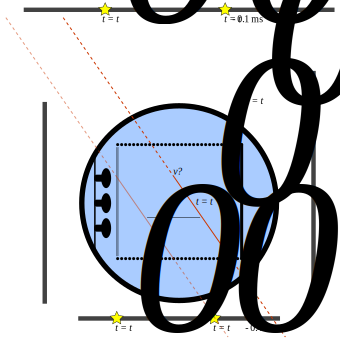
\includegraphics[width=1.0\textwidth]{images/MicroBooNE/CRTTrackAssociation.pdf}
    \caption[CRT Track Association]{This is a schematic view of the track association strategy used in MicroBooNE. The yellow stars represent \gls{crt} particle hits. The opaque solid red line is the \gls{tpc} particle track, with an apparent \gls{Vertex} at $t = t_0$. The semitransparent red line is the same track shifted to the readout time $t=t_0+\SI{1.3}{\milli\second}$, coinciding with a \gls{crt} hit at the bottom plane. The dashed lines, are the likely extensions of the track. Above depiction is inspired by \cite{CRTThomasPhD}.}
    \label{fig:CRTTrackAssociation}
\end{figure}
Thereby, the \gls{tpc} charge readout window gets shifted in to the timestamps of every \gls{crt} particle hit. For all tracks their likely extension is calculated, \ie the direction of the track at both ends gets extended outside of the \gls{tpc}. Now, if these likely extension intersect with a \gls{crt} hit, the \gls{tpc} track and the \gls{crt} hit get associated, or in other words, the track gets tagged by the \gls{crt}. With this method the matching efficiency in MicroBooNE is about \SI{50}{\percent}, \ie half of cosmic induced tracks registered by the \gls{tpc} can be associated to a \gls{crt} hit. This is mainly attributed to the limited coverage of the systems, as there are large gaps between the top and the side panels as well as missing upstream and downstream planes. The contribution of reconstruction inefficiencies and \gls{crt} dead times are expected to be marginal in comparison \cite{CRTThomasPhD}.

As mentioned before at the end of section \ref{sec:MicroBooNEReadout}, MicroBooNE's neutrino trigger is the coincidence of a \gls{bnb} beam pulse trigger and a scintillation \gls{Flash} in this \gls{BeamGate} of \SI{1.6}{\micro\second}. This trigger logic has one major background, when a cosmic induces the \gls{Flash} instead of a beam event. In fact, it is more likely that a cosmic particle is responsible for the \gls{Flash} than a neutrino. To mitigate this issue, the \gls{crt} can also be used as a veto. This is done, by discarding all events if the trigger \gls{Flash} in the \gls{lartpc} coincides with a \gls{crt} hit. There is a catch though: If one of the daughter particles of a neutrino interaction leaves the \gls{tpc} and creates a \gls{crt} hit, the veto will discard an actual event. However, this occurrence is rare and quantifiable \cite{CRTThomasPhD}.

% TODO put this section above CRT? Maybe not because of the readout stuff, that lines up nicely between the TPC and CRT section
\section{Laser Calibration System} \label{sec:LaserCalibrationSystem}
As touched on before in section \ref{sec:MultiPhotonIonisation}, \gls{uv}-laser systems are excellent standard track generators for a \gls{lartpc}. They can be used to measure drift field distortions, the \textbf{oxygen equivalent impurity level}, as well as other detector calibration quantities. The foundation for MicroBooNE's \gls{lcs} was laid 2009, when the \gls{lar} group at \gls{lhep} started - and I quote: \cite[\textit{the development of a novel online monitoring and calibration system exploiting UV-laser beams}]{LArLaserLHEP}. This system was improved upon and used in Argontube, wherein it was used in a large scale detector for the first time with ionisation tracks of about \SI{5}{\metre} length \cite{Argontube3}. Finally, the development culminated in the \gls{lcs} installed in MicroBooNE \cite{LArLaserMicroBooNE1,LArLaserMicroBooNE2}, where I played a vital part in its conception and the software reconstruction efforts. Its main goal is to measure and calibrate for the expected electric field inhomogeneities in the \gls{lartpc}. The calibration itself was eventually performed by M. L\"uthi and Y. Chen and is documented in their respective PhD thesis \cite{LArLaserPhDMatthias,LArLaserPhDYifan}. This section here is merely a summary of the work of these two colleagues.

\subsection{Laser Head and Beam Optics}
The name laser was originally an acronym, \textbf{L}ight \textbf{A}mplification by \textbf{S}timulated \textbf{E}mission of \textbf{R}adiation, which became a word in the years following its invention \cite{LaserFirst}. The centrepiece of a laser is the so-called \textbf{gain medium}, usually a crystal rod. The atoms of said crystal are excited by an external light source. When these excited states decay, they emit monochromatic light longitudinally to the rod, all while the external light source produces new excited states. The crystal is placed between two mirrors, one of them partially transparent, forming the so-called \textbf{cavity}. As the laser photons are reflected at either end of the cavity, they pass through the crystal again. Thereby, they stimulate the emission of further photons which feature the same wavelength, move in the same direction and are in phase with one another, \ie the photons are \textbf{coherent}. With every passage through the gain medium, the laser gains intensity until the number of photons becomes so great, that they pass through the partially transparent mirror. Above description of a laser is quite simplistic and for more detailed information consider \cite{LaserTheory}. 

The core of MicroBooNE's \gls{lcs} is constituted by two Surelite\textsuperscript{\texttrademark} SL I-10 laser heads manufactured by Continuum\textsuperscript{\textregistered} \cite{LaserManual}. The specifications of a Surelite SL I-10 laser are listed below in table \ref{tab:LaserProperties}.
\begin{table}[hbt]
	\centering
    \caption[Specifications of the Surelite SL I-10 Laser at \SI{266}{\nano\metre}]{Specifications of the Continuum\textsuperscript{\textregistered} Surelite\textsuperscript{\texttrademark} SL I-10 laser at \SI{266}{\nano\metre} \cite{LaserManual}. The optical power and peak optical intensity of a single laser pulse are calculated values assuming a Gaussian pulse profile using equations \ref{eq:PulsePower}, \ref{eq:OptialIntensity}, and \ref{eq:LaserFieldStrength}; the latter two with $w = w_0$. They both are given in a range, since they depend on the pulse width.}
    \label{tab:LaserProperties}
	\begin{tabu}{lrl}
        \toprule
        Laser Property & Value & Unit \\
        \midrule
        Maximum pulse rate & \num{10} & \si{\hertz} \\
        Energy per pulse $E_\text{p}$ & \num{60} & \si{\milli\joule} \\
        Beam diameter $w_0$ & \num{6} & \si{\milli\metre} \\
        Linewidth & \num{1} & \si{\per\centi\metre} \\
        Beam divergence & \num{0.5} & \si{\milli\radian} \\
        Pulse width $\tau_\text{p}$ & \numrange{4}{6} & \si{\nano\second} \\
        \midrule
        Energy stability (RMS) & \num{+-2.3} & \si{\percent} \\
        Power drift ($\Delta T < $\SI{+-3}{\degreeCelsius}) & \num{+-8} & \si{\percent}  \\
        Jitter & \num{+-0.5} & \si{\nano\second} \\
        Beam pointing stability  & \num{+-30} & \si{\micro\radian} \\
        \midrule
        \multicolumn{2}{l}{Beam spatial profile (1.0 for a Gaussian beam)} & \\
        \qquad Near field (\SI{<1}{\metre}) & 0.70 & \\
        \qquad Far field ($\infty$) & 0.95 & \\
        \midrule
        Optical power $P$ (calculated) & \numrange[separate-uncertainty = false]{9.4(2)}{14.1(3)} & \si{\mega\watt} \\
        Peak optical intensity $I_0$ (calculated) & \numrange[separate-uncertainty = false]{16.6(4)}{24.9(6)} & \si{\mega\watt\per\centi\metre} \\
        Peak electric field strength $F$ (calculated) & \numrange[separate-uncertainty = false]{91.3(21)}{112(3)} & \si{\kilo\volt\per\centi\metre} \\
        \bottomrule
    \end{tabu}
\end{table}
This type is a high energy (class 4) \gls{ndyag} laser with a base wavelength of \SI{1064}{\nano\metre}. To generate triggered pulses, the laser head makes use of a so-called \textbf{active Q-switch}. For Q-switching, the \gls{ndyag} crystal rod is constantly pumped by a water cooled xenon flashlamp, which ensures a high level of energy being stored. Then, a modulator is incorporated into the laser cavity, introducing losses by diffraction, which inhibits the pulse formation. Once a trigger signal arrives, the state of said modulator is changed and with it the losses are stopped. Consequently, the energy stored in the laser cavity is released in a pulse \cite{LaserBasics2}. Surelite's Q-Switch is realised with a combination of a \textlambda/4-\gls{Waveplate}, a \gls{PockelsCell}, and a polariser \cite{LaserManual}. As can be seen from figure \ref{fig:LaserHead}, the beam passes through the Q-Switch complex twice, once from the laser head side and then backwards after reflecting off the rear mirror. The light produced in the \gls{ndyag} crystal is horizontally, \ie p-polarised, and can pass through the polariser without interference. After passing through the \textlambda/4-\gls{Waveplate}, the polarisation is circular. Now, if the \gls{PockelsCell} is not powered, the circularly polarised light is simply reflected back to the \gls{Waveplate} where it is converted to a vertical, \ie s-polarisation. However, this light is not able to pass the polariser and is thus reflected to the side. Hence, no laser pulse is produced and we speak of a closed cavity. Now if a voltage of $\sim\SI{3.6}{\kilo\volt}$ is applied, the \gls{PockelsCell} is able to flip the polarisation by an additional $\pi/2$ and thus we get again p-polarised light after the second pass through the \textlambda/4-\gls{Waveplate}. Hence the light is allowed to pass the polariser, \ie the cavity is open \cite{LaserTheory,LaserManual}. Finally a \gls{GaussianMirror} completes the laser cavity.
\begin{figure}[htbp]
    \centering
    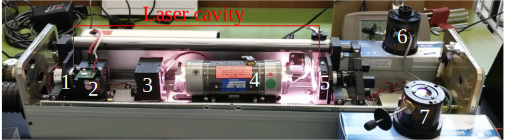
\includegraphics[width=1.0\textwidth]{images/MicroBooNE/LCSLaserHead.pdf}
    \caption[LCS Laser Head]{Shown above is a photograph of the open and partially disassembled Surelite SL I-10 laser head. Positioned at (1) is the rear mirror, at (2) the \gls{PockelsCell}, at (3) we find the \textlambda/4-\gls{Waveplate} and polariser assembly, (4) is the water cooled xenon flashlamp assembly containing the \gls{ndyag} crystal rod, and finally at (5) the \gls{GaussianMirror} completes the laser cavity. The numbers (2) and (3) form the Q-Switch of the Surelite. Furthermore, there are the two nonlinear crystals (6) and (7), used for frequency quadrupling, moved to the side. Usually they would be installed in the beam line after the \gls{GaussianMirror}. This picture was taken by Y. Chen and sourced from her thesis \cite{LArLaserPhDYifan}.}
    \label{fig:LaserHead}
\end{figure}
As mentioned above, the wavelength of an \gls{ndyag} laser is \SI{1064}{\nano\metre}, and hence, in the near-infrared. In order to generate a \gls{uv} beam, the raw laser output is coupled into nonlinear crystals. In these crystals, the beam induces an oscillating polarisation which, due to the non-linearity, features a component with twice the input frequency. Such nonlinear crystals are usually made of lithium triborate, \ce{LiB3O5} \cite{LaserBasics1}. After this frequency doubling, also called \textbf{second-harmonic generation}, we are not left with monochromatic light, but a mix of the input and the doubled frequency. In the case of the \gls{lcs}, second-harmonic generation is performed twice, once to \SI{532}{\nano\metre} and then again to \SI{266}{\nano\metre}, leading to a frequency quadrupling or fourth-harmonic generation. The two crystals are also shown in figure \ref{fig:LaserHead}.

After leaving the laser head, the beam is first reflected by a \gls{DichroicMirror}, whereby the beam residuals with \SIlist{1064;532}{\nano\metre} wavelength are partially filtered and mostly the \SI{266}{\nano\metre} photons are reflected. Thereafter, the beam is guided through the ALTECHNA Watt Pilot attenuator \cite{LCSAttenuator}. This device consists of a rotating \textlambda/2-\gls{Waveplate}, which linearly polarises the beam, and two thin film polarisers installed at their \glspl{BrewsterAngle}. With this, the s-polarised beam component are reflected while the p-polarised components are transmitted through the material. The attenuator produces two parallel beams, each with a different \glspl{LinearPolarisation}. The attenuation factor of the laser beam is then given by the position of the \textlambda/2 wave plate, which defines the intensities of s- and p-polarised light. Then, the p-polarised beam is passed through a motorised aperture used to reduce the beam spot size, whereas the s-polarised beam is dumped. Thereafter the beam is reflected by another \gls{DichroicMirror} in a motorised mirror holder, facilitating remote adjustments of the beam direction. In addition a visible alignment laser is coupled into the beam line through the backside of the first \gls{DichroicMirror}. This laser proved to be useful for achieving a pre-alignment of the beam over the relatively large distances found in the MicroBooNE \gls{lcs}. During regular laser operations the alignment laser is deactivated. In order to get a trigger signal for the MicroBooNE readout electronics, see section \ref{sec:MicroBooNEReadout}, a photodiode produced by Thorlabs is employed. This photodiode catches stray light from the laser setup and creates an analogue signal. This signal is then binarised by a \gls{Discriminator} and sent to MicroBooNE's trigger board. A schematic view of this optical setup is given in figure \ref{fig:BeamOptics}.
\begin{figure}[hbtp]
    \centering
    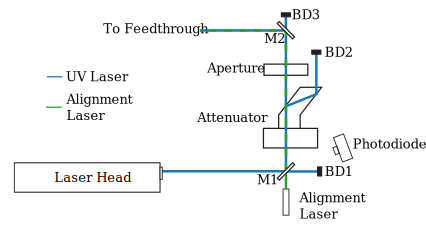
\includegraphics[width=0.9\textwidth]{images/MicroBooNE/LCSBeamOptics.pdf}     
    \caption[LCS Beam Optics]{Shown above is a schematic view of the \gls{lcs} beam optics enclosed in the laser box. The two \glspl{DichroicMirror} are labelled with M1 and M2. The Pieces named BDx are beam dumps made of corrugated Teflon plates. The left beam leaving the attenuator is p-polarised, while the right beam ending in BD2 is s-polarised. The original of above depiction was created by M. L\"uthi \cite{LArLaserPhDMatthias} and adapted for this work.}
    \label{fig:BeamOptics}
\end{figure}
All of the abovementioned optical components as well as the laser head are contained in a light-tight laser box, which is \SI{2}{\metre} long, \SI{0.5}{\metre} wide, and \SI{0.5}{\metre} high and shown in figure \ref{fig:LaserBox}. Two of these boxes are installed on top of the cryostat on a table-like structures. After leaving the laser box, each beam is guided through an enclosed beam pipe to their respective laser feedthrough, which will be discussed next.
\begin{figure}[htbp]
    \centering
    \includegraphics[width=1.0\textwidth]{images/MicroBooNE/LCSLaserBox.pdf}     
    \caption[LCS Laser Box]{This picture shows the opened laser box (1) containing the laser head (2). The tower with the vertically mounted beam optics carries the number (3), and on top of it one finds the motorised \gls{DichroicMirror} (4). The photodiode can be seen at (5). During laser operations, this box is sealed with a top cover.}.
    \label{fig:LaserBox}
\end{figure}

\subsection{Laser Feedthrough} \label{sec:LaserFeedthrough}
The purpose of the laser feedthrough is to guide the \gls{uv} laser beam from air into \gls{lar} and the therein immersed \gls{tpc}. Note, we distinguish two areas of the feedthrough: the \textbf{warm part} in air and the \textbf{cold part} immersed in \gls{lar}. In order to initiate the transition from warm part to cold part, a motorised \gls{DichroicMirror} by Edmund Optics, optimised for \SI{266}{\nano\metre} wavelengths, is situated on top of the feedthrough. This so-called \textbf{warm mirror} reflects the laser beam vertically downwards into the cryostat. An evacuated quartz glass tube acts as optical interface between the air an \gls{lar}. The laser beam passes through this tube and into the \gls{lar}, where it is reflected again by a mirror at the bottom of the feedthrough. This so-called \textbf{cold mirror} is the same type as the warm mirror and it too is steerable. Through the gaps between field cage loops, the laser is able to enter the \gls{lartpc} and leave multiphoton ionisation tracks, as discussed in section \ref{sec:MultiPhotonIonisation}. Since there are two systems, the above-described path is available from the upstream and the downstream end of the detector. The optical path of the feedthrough setup is shown in figure \ref{fig:FeedthroughOptics}. 
\begin{figure}[htbp]
    \centering
    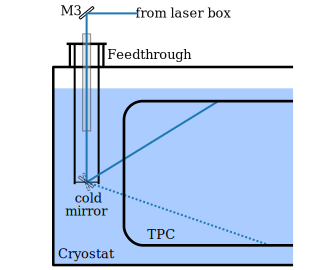
\includegraphics[width=0.8\textwidth]{images/MicroBooNE/LCSFeedthroughOptics.pdf}     
    \caption[LCS Feedthrough Schematics]{Shown here is a schematic view of the laser beam's optical path through the feedthrough setup. This figure is sourced from \cite{LArLaserPhDMatthias}.}
    \label{fig:FeedthroughOptics}
\end{figure}
Both \glspl{DichroicMirror} used at the feedthrough are optimised for air as its surrounding medium. These mirrors employ thin films with different refractive indices to achieve a wavelength optimised reflectivity for both \glspl{LinearPolarisation}. Hence, reflectivity issues arise when they are moved from air with a refracting index of $n \approx \num{1}$ to \gls{lar} with an expected $n \approx \num{1.3}$ at a wavelength of \SI{266}{\nano\metre} \cite{LArRefractiveIndex,LArLaserPhDMatthias}. A simulation by Edmund Optics indeed showed a reduced reflectivity at large angles of incidence, see figure \ref{fig:MirrorReflectivity}.
\begin{figure}[htbp]
    \centering
    \includegraphics[width=1.0\textwidth]{images/MicroBooNE/LCSReflectionAngles.pdf}     
    \caption[Cold Mirror Reflectivity]{This graph shows the reflectivity of the cold mirror immersed in \gls{lar} as a function of the angle of incidence. Said angle is defined from perpendicular to the mirror surface at \SI{0}{\degree} to parallel to the surface at \SI{90}{\degree}. The graph is sourced from \cite{LArLaserPhDMatthias}.}
    \label{fig:MirrorReflectivity}
\end{figure}
More specifically, the simulation shows a major drop in the cold mirror's reflectivity for a s-polarised \gls{uv} laser beam already around a \SI{45}{\degree} angle of incidence. This would mean that the laser beam could not be reflected to the lower parts of the \gls{tpc}. For a p-polarised beam, said drop occurs for an angle of incidence beyond \SI{60}{\degree}. This is the reason for choosing the p-polarised beam originating from the attenuator.

As \gls{lhep} joined the MicroBooNE collaboration quite late, when the cryostat design was almost finalised, there were only two spare nozzles available. They are positioned on each end cap of the cryostat, slightly off the centre line, and feature a \gls{cf} \num{100} flange. These circumstances certainly made the laser feedthrough the major technical challenge of the \gls{lcs}, as it has to fulfil the following requirements and constraints:
\begin{enumerate}
    \item Optically couple the laser beam from air into \gls{lar} to minimise beam intensity losses and prevent scattering
    \item Actively steer the beam with a mirror immersed in \gls{lar} on two axis to ensure adequate beam coverage in the \gls{lartpc}
    \item Accurately determine the mirror angle in both axis for true track calibration, see section \ref{sec:SpaceCharge} 
    \item Containing no metal parts in \gls{lar} because of the close proximity to the field cage
    \item Withstand the extreme temperature gradient between room temperature and \SI{87}{\kelvin} in a short distance
    \item Be vacuum tight to maintain \gls{lar} purity
    \item Withstand MicroBooNE's rated maximum overpressure of \SI{2.1}{\bar} for safety reasons
\end{enumerate}
The very first requirement was already fulfilled by the design of \gls{lhep}'s first static laser feedthrough \cite{LArLaserLHEP}, which employs the aforementioned closed and evacuated quartz glass tube. Said tube is immersed into \gls{lar} and hence a smooth surface interface is created by the glass window at the end of the tube. The vacuum applied to the tube acts as thermal insulator and prevents condensation. This glass tube is held in place by three rubber seals separated by metal rings, which are incorporated into a \gls{cf} flange. When these rings are compressed, the seals squeeze against the tube and ensure vacuum tightness. The implementation of a two axis movement of the cold mirror, on the other hand, had to be conceived from scratch. Certainly, a direct motorisation using cryogenic motors would have been the easiest option. However, the close proximity of the field cage and its \gls{hv} prohibited such a setup. Thus, we had to come up with an indirect scheme utilising motorised feedthroughs, all while keeping the setup vacuum tight and overpressure resilient.

Providing the horizontal movement of the cold mirror, is a rotational feedthrough manufactured by Thermionics, type RNN-400. Its rotation provides beam steerability in the $x$-$z$-plane in the MicroBooNE coordinate system, consider figure \ref{fig:MicroBooNECoordinateSystem}. Aforementioned rotational feedthrough features three circular ceramic seal enclosing two cavities which are differentially pumped, in order to maintain the vacuum tightness. The movement is induced by a stepper motor and transmitted to the feedthrough via a worm drive. The rotation angle is measured by a Heidenhain AK ERA 4480 rotary encoder providing a accuracy of \SI{0.001}{\degree} \cite{LArLaserPhDMatthias}. The vertical movement, \ie beem steerability in the $y$-$z$-plane, is introduced by a Thermionics FLMR-133-25 Series vacuum sealed linear actuator. It too is powered by a stepper motor and its position is measured by a Heidenhain LC 415 linear encoder with an accuracy of \SI{1}{\micro\metre}. The above described setup is shown in figure \ref{fig:FeedthroughHead}.
\begin{figure}[htbp]
    \centering
    \includegraphics[width=1.0\textwidth]{images/MicroBooNE/LCSFeedthroughTop.pdf}     
    \caption[LCS Feedthrough Top]{This photograph shows the top part of the \gls{lcs} feedthrough. Marked with (1), we find the motorised \gls{DichroicMirror} (M3 in figure \ref{fig:FeedthroughOptics}) used to reflect the beam down into the feedtrough. (2) marks the quartz glass tube holding structure, (3) is the stepper motor of the rotational feedthrough, while (4) is the gear of the worm drive. (5) shows the rotary encoder ring and (6) the holding structure of the encoder sensor. Positioned at (7) is the other stepper motor and at (8) the linear actuator. Finally, (9) is the holding structure of the linear encoder.}
    \label{fig:FeedthroughHead}
\end{figure}
The quartz glass tube is mounted on the optical axis in the centre of rotation of the feedthrough. The above-described warm part of the feedthrough is also encased in a light-tight cylindrical enclosure, not shown in the figure.

Mounted underneath the rotating part of the feedthrough, one finds the cold mirror support structure made of Duratron\textsuperscript{\textregistered} T4301 \cite{LArLaserPhDMatthias}, a \gls{pai}. Said rigid structure is composed of ten \SI{15}{\centi\metre} long, almost identical segments. Every segment consisting of four cylindrical rods and a horizontal connector plate in the shape of an open ring. These plates not only increase stability, but also provide a guide for the steering rod of the cold mirror. Said cold mirror is mounted in the centre of the last \gls{pai} segment, in a inclinable holding structure featuring a half-pinion on its backside. The aforementioned steering rod features a rack at the cold mirror's height. Consequently, the linear movement of the actuator is translated into tilting motion of the mirror by means of a rack and pinion drive. The change in tilting angle $\Delta\alpha$ can be calculated with the formula
\begin{equation}
    \Delta\alpha = \frac{1}{s} \Delta L,
\end{equation}
where $\Delta L$ denotes the linear movement, and $s$ the transmission ratio. The latter was measured as $s = \SI[per-mode = symbol]{ 0.3499(2)}{\milli\metre\per\degree}$ \cite{LArLaserPhDMatthias}. Applying above formula to the linear readout accuracy, we get an angular accuracy of the tilt movement of \SI{0.003}{\degree}. In the MicroBooNE coordinate system the two cold mirror centres are located at $(x,y,z) = (\num{103.8},\num{8.6},\num{-35.6})$ (upstream system), and $(\num{102.5},\num{8.2},\num{1080.2})$ (downstream system), respectively \cite{LArLaserMicroBooNE2}. Pictures of a fully assembled \gls{lcs} feedthrough are shown in figure \ref{fig:FeedthroughPictures}. In order to prevent potential electrical noise in the \gls{tpc} readout systems induced by the motors, the rotary feedthrough is insulated from the cryostat by a ceramic circuit breaker (see bottom of the feedthrough in figure \ref{fig:FeedthroughTop}). Moreover, all parts immersed in \gls{lar} are fastened by non-conductive \gls{pai} screws, in avoidance of possible \gls{hv} breakdowns of the field cage, see figures \ref{fig:FeedthroughBottom} and \ref{fig:ColdMirror}.
\begin{figure}[htbp]
    \centering
    \resizebox{\textwidth}{!}{
    \subfloat[Warm Part][Warm part]
    {
        \includegraphics[height=10cm]{images/MicroBooNE/LCSFTWarmPart.png} 
       \label{fig:FeedthroughTop}
    } 
    \subfloat[Cold Part][Cold part]
    {
        \includegraphics[height=10cm]{images/MicroBooNE/LCSFTColdPart.png}
        \label{fig:FeedthroughBottom}
    } 
    \subfloat[Cold Mirror Mount][Cold mirror mount]
    {
        \includegraphics[height=10cm]{images/MicroBooNE/LCSFTColdMirror.png}
        \label{fig:ColdMirror}
    }
    }
    \caption[Fully assembled LCS Feedthrough]{Above pictures show a fully assembled feedthrough on a test mount. The top of the feedthrough assembly, or warm part, is shown in \subref{fig:FeedthroughTop}. In \subref{fig:FeedthroughBottom} the same feedthrough is shown from the bottom up. This so-called cold part is made of \gls{pai} and is there to hold the cold mirror. At last, \subref{fig:ColdMirror} shows the cold mirror with its rack and pinion drive, converting the vertical motion of a linear actuator into a mirror rotation.}
    \label{fig:FeedthroughPictures}
\end{figure}

\subsection{Field Calibration Results}
As stated above, the \gls{lcs} was primarily conceived for the study of electric field distortions due to space charge. Using the methods described in section \ref{sec:SpaceCharge}, we were able to measure the spacial displacement, drift velocity, and with it the electric field in most of the regions of MicroBooNE's \gls{lartpc}. As the latter two exhibit almost a perfect linear dependency, when considering a small enough interval (see figure \ref{fig:DriftVelocity}), only the electric field and the displacement is discussed here. Both these measured entities are stored in \gls{3d} maps, whereby a \gls{3d} vector is located at any given space point of said map. Such a complex construct of a vector field is quite difficult to visualise. Hence, it is favourable to only show \gls{2d} slices, or in other words a sectional view. In MicroBooNE the required slicing cuts are made perpendicular to the $z$-axis, meaning the \gls{2d} representation is shown in the $x$-$y$-plane at a respective $z$-coordinate. Moreover, the three components of the respective vector are depicted in separate graphs accordingly.

A slice of the displacement map is shown in figure \ref{fig:Displacement}. The depicted slice's position is in the centre of MicroBooNE's $z$-coordinate at $z=\SI{518}{\centi\metre}$. The axis show the $x$, and $y$ position, while the colour axis shows the displacement in centimetres, as defined by equation \ref{eq:DisplacementDefinition}. For the measurement itself the reconstructed space points of all the recorded laser tracks were divided into \num{50} subsets which are then interpolated separately. Lastly, the resulting \num{50} interpolated regular grid maps are averaged. This procedure not only solves computing issues, but also enables an uncertainty analysis. The statistical uncertainty of the displacement slice is shown in \ref{fig:DisplacementError}. These uncertainties are determined by calculating the standard deviation of these \num{50} subsets.
\begin{figure}[htbp]
    \centering
    \subfloat[Displacement Slice][Displacement slice]
    {
        \includegraphics[width=1.0\textwidth]{images/MicroBooNE/LCSDisplacementMap.pdf}
        \label{fig:Displacement}
    } \\
    \subfloat[Displacement Statistical Uncertainty Slice][Statistical uncertainty slice]
    {
        \includegraphics[width=1.0\textwidth]{images/MicroBooNE/LCSDisplacementMapError.pdf}
        \label{fig:DisplacementError}
    }
    \caption[Measured Displacement in MicroBooNE using the LCS]{Above graphs show a slice of the displacement map, measured using the \gls{lcs}. The slice in question is a $y$-$z$-plane view in the centre of the $z$-axis at $z=\SI{518}{\centi\metre}$. In \subref{fig:Displacement}, from left to right the displacement in the $x$, $y$, and $z$-direction are shown on the colour axis in centimetre. In \subref{fig:DisplacementError}, the statistical uncertainty, \ie standard deviation, of the same slice is shown also in centimetre. Both graphs are sourced from \cite{LArLaserMicroBooNE2,LArLaserPhDYifan}.}
    \label{fig:LCSDisplacementMaps}
\end{figure}
As can be seen from this central slice, the maximum displacement in $x$-direction amounts to $\sim\SI{4}{\centi\metre}$, $\sim\SI{15}{\centi\metre}$ in $y$-direction, and $\sim\SI{0.2}{\centi\metre}$ in $z$-direction. The corresponding statistical uncertainties are in the range from \SIrange{0.1}{2.5}{\centi\metre}.

The drift electric field map slice corresponding to the displacement slice at $z=\SI{518}{\centi\metre}$ is shown in figure \ref{fig:ElectricField}. To arrive at this slice, the full \gls{3d} displacement map first had to be converted to a velocity field map, in accordance with equation \ref{eq:VelocityDistortion}. From there the electric field was obtained by solving the mobility relation of equation \ref{eq:DriftVelocity}. For the electric field slices, it is suitable to present the field deviation as a fraction of the undisturbed field $E_0$. Said fractions are represented by the colour axis on the graphs. Naturally, said field deviation with respect to the undisturbed state are given by $E_x-E_0$, $E_y$, and $E_z$, respectively. Furthermore, the corresponding uncertainties of these electric field deviation fractions are depicted in figure \ref{fig:ElectricFieldError}. These statistical uncertainties are obtained by error propagation of the displacement map. Lastly, there are also systematic uncertainties which are determined by reconstructing a known field generated by a space charge simulation \cite{LArLaserMicroBooNE2}. The difference between the simulated electric field strength and the reconstructed one, \ie $\vec{E}^{\text{sim}} - \vec{E}^{\text{calc}}$, is then taken as the systematic uncertainty. In order to make it comparable to the other slices, said difference is also divided by $E_0$. The systematic uncertainty of the central detector slice is shown in figure \ref{fig:ElectricFieldSystematics}.
\begin{figure}[htbp]
    \centering
    \subfloat[Drift Electric Field Slice][Drift electric field slice]
    {
        \includegraphics[width=1.0\textwidth]{images/MicroBooNE/LCSFieldMap.pdf}
        \label{fig:ElectricField}
    } \\
    \subfloat[Electric Field Statistical Uncertainty Slice][Electric field statistical uncertainty slice]
    {
        \includegraphics[width=1.0\textwidth]{images/MicroBooNE/LCSFieldMapError.pdf}
        \label{fig:ElectricFieldError}
    }\\
    \subfloat[Electric Field Systematic Uncertainty Slice][Electric field systematic uncertainty slice]
    {
        \includegraphics[width=1.0\textwidth]{images/MicroBooNE/LCSFieldMapSystematics.pdf}
        \label{fig:ElectricFieldSystematics}
    }
    \caption[Measured Drift Electric Field in MicroBooNE Using the LCS]{A slice at $z=\SI{518}{\centi\metre}$ of the three components of the drift electric field map measured in MicroBooNE are depicted from left to right. On the colour axis in \subref{fig:ElectricField}, deviation of the field component with respect to the expected drift field value $E_0$ is given. This means $(E_x-E_0)/E_0$ on the left, $E_y/E_0$ in the middle, and $E_z/E_0$ on the right, all in units of percent. In \subref{fig:ElectricFieldError} the statistical uncertainties relative to $E_0$ are shown, \ie $\sigma(E_x)/E_0$, $\sigma(E_z)/E_0$, and $\sigma(E_z)/E_0$. Finally, in \ref{fig:ElectricFieldSystematics} the systematic uncertainties are depicted, \ie $(E_x^{\text{sim}} - E_x^{\text{calc}})/E_0$, $(E_y^{\text{sim}} - E_y^{\text{calc}})/E_0$, $(E_z^{\text{sim}} - E_z^{\text{calc}})/E_0$. These graphs are also sourced from \cite{LArLaserMicroBooNE2,LArLaserPhDYifan}.}
    \label{fig:LCSFieldMaps}
\end{figure}
In the central slice, the ratios of $(E_x-E_0)/E_0$ and $E_y/E_0$ show a maximum value of $\sim\SI{15}{\percent}$, while $E_z/E_0$ shows a maximum of $\sim\SI{2}{\percent}$. The relative statistical uncertainties, \ie $\sigma(E_x)/E_0$, $\sigma(E_z)/E_0$, and $\sigma(E_z)/E_0$, all show similar maxima at $\sim\SI{5}{\percent}$, although they typically are below \SI{2}{\percent} when disregarding the areas close to the cathode. Finally, the relative systematic uncertainties, \ie $(\vec{E}^{\text{sim}} - \vec{E}^{\text{calc}})/E_0$, are roughly of the same order as the statistical uncertainties. Note, that the characteristics of a \gls{1d} representation of $(E_x-E_0)/E_0$ along the $x$-axis at $y = 0$ resembles the model predicted curve in figure \ref{fig:SpaceChargeField}. As expected the term $E_x-E_0$ is negative at the anode, curving upwards to $E_x-E_0 = 0$ at around $x=\SI{150}{\centi\metre}$, and reaching its maximum at the cathode.

% TODO what can be improved with these maps? Better vertex location shown in Yifan's thesis. Maybe not...
% TODO maybe criticism: ambiguities, wonky systematics with the wrong simulation...
